\documentclass[a4paper,openright, 14pt]{article}
\usepackage[utf8]{inputenc}
\usepackage{graphicx}
\usepackage{tikz}
\usetikzlibrary{datavisualization}
\usetikzlibrary{datavisualization.formats.functions}

\graphicspath{ {./images/} }

\usepackage{fullpage}
\newcommand{\ssection}[1]{%
\section[#1]{\centering\normalfont\scshape #1}}
\newcommand{\ssubsection}[1]{%
\subsection[#1]{\bfseries\normalfont\scshape #1}}
\newcommand{\ssubsubsection}[1]{%
\ssubsubsection[#1]{\bfseries\normalfont\scshape #1}}

\title{Study Guide}
\author{Team L.A.J., League of Anti Josh}
\date{Quarter 2}

\begin{document}

\maketitle
\section*{Table of Contents}

\ssection{Parametric Equations}
 \section*{Introduction}
 When we usually plot x and y coordinates, there's only one equation that shows the relationship between x and y. To solve this equation, we'd want to isolate y and get it in terms of x. This is called a rectangular equation. This is very limiting and allows us to only see x and y as they relate to each other. An example of a rectangular equation would be $y=2x$ or $y=x^2-x+2$. The equation, $y=2x$, would look like this:
 \begin{center}
     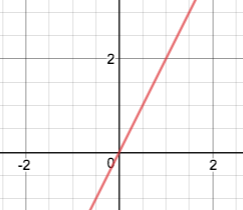
\includegraphics[width =4 cm, height= 3 cm]{Images/graph1.png}
 \end{center}
 Parametric equations, however, are x and y equations in terms of t. They still allow us to plot x and y, but they're independent of each other. This can allow us to graph certain shapes that rectangular equations wouldn't allow us to, such as a circle or spiral. Now, let's try graphing some of these equations.
 \section*{Graphs}
 In order to graph parametric equations, all we have to do is choose some t values, substitute them into the x and y equations, and think about what this means for the overall pattern of the graph. When you substitute in a t value, a y and an x value are created, and you plot them on an xy plane. This shows a path of motion and how a graph moves. Let’s try it out with a couple examples. 

\\\\
\underline{Example 1}\\
$$x(t)=t,y(t)=t$$
Given this, sub in t values to give a general idea of what this graph is going to look like. First substitute in $t=1$
$$t=1$$
$$y=1$$
$$x=1$$
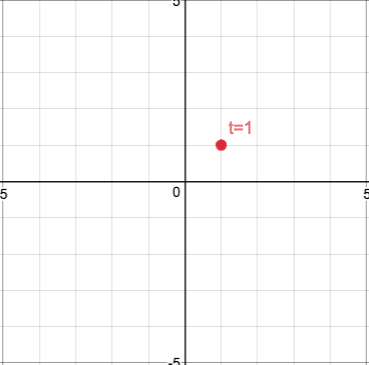
\includegraphics[width = 5 cm, height = 5 cm]{JOSHUA2.png}\\
\\Now that we have our first point lets try and substitute a bit more and show a path of motion on a graph.\\\\
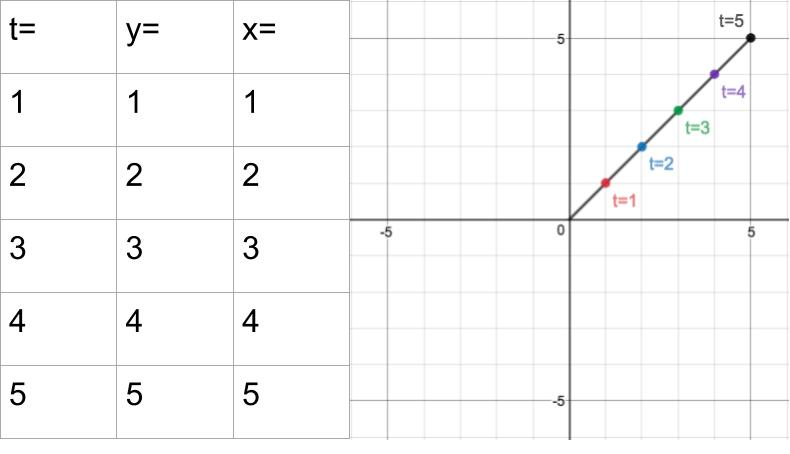
\includegraphics[width = 15 cm, height = 7 cm]{JOSHUA1.jpg}\\
As you can see the graph begins at the origin and moves its way up as more and more t values exist. Lets try going backwards with t by putting in negative values. \\
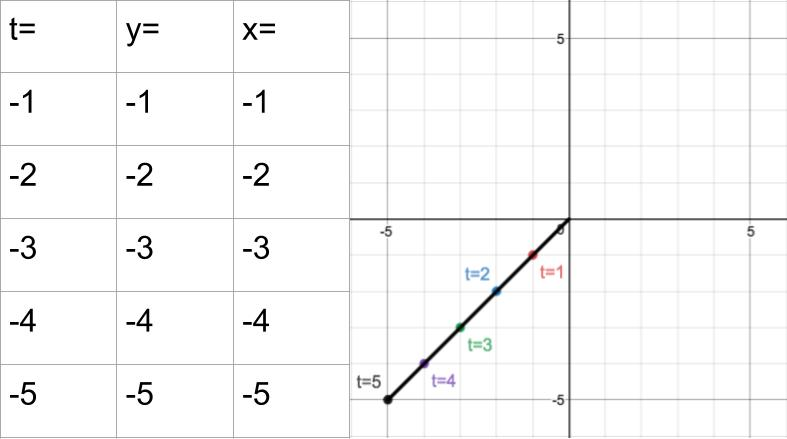
\includegraphics[width = 15 cm, height = 7 cm]{JOSHUA3.jpg}\\
As t is negative the path of motion seems to be going into the opposite direction.\\
\\\\
\underline{Example 2}\\
Lets examine a circle and how its path of motion works.\\
Your circular equation in xy form is going to be...
$$x^2+y^2=25$$
Now we cannot find the path of motion with x and y so we will have to make a t substitution. Let's say $y=xt$.
$$x^2+y^2=25$$
$$x^2+(xt)^2=25$$
$$x^2+ t^2 x^2=25$$
Factor out an $x^2$ and divide by the other factor.
$$x^2+ t^2 x^2=25$$
$$x^2(1+ t^2)=25$$
$$x^2=\frac{25}{1+t^2}$$
Now square root both sides.
$$x=\pm \sqrt{\frac{25}{1+t^2}}$$
Don't forget to substitute back into y(t).
$$y=xt$$
$$y=\pm t \sqrt{\frac{25}{1+t^2}}$$
Now we have two new parametric equations for the circle. Let's see what happens when we graph them.
$$y=t \sqrt{\frac{25}{1+t^2}}$$
$$x=\sqrt{\frac{25}{1+t^2}}$$
We shall again plot using a graph from $-5<t<5$\\
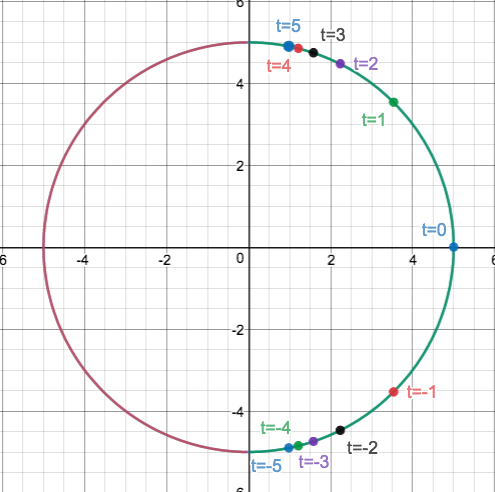
\includegraphics[width = 7 cm, height = 7 cm]{JOSH.png}\\
This graph only gives us half of what the original graph was. As you approach negative infinity you'll get to the bottom of the circle and as you approach positive infinity you'll hit the top of the circle. We can predict that if we were to use the negative part of x(t) that it would be the other half of the circle with similar path of motion.\\\\
We can use a different substitution however to gain a different path of motion for the same equation. Let's say that $1=cos^2 (t) + sin^2(t)$ and lets try to get 1 in terms of x and y in our original equation.
$$x^2 +y^2=25$$
$$\frac{x^2}{5^2} +\frac{y^2}{5^2}=1$$
Now substitute in $1=cos^2 (t) + sin^2(t)$.
$$\frac{x^2}{5^2} +\frac{y^2}{5^2}=cos^2 (t) + sin^2(t)$$
Think about how x coordinates with cosine and how y coordinates with sine. Set $x^2/5^2=cos^2(t)$ and solve.
$$x^2=5^2cos^2(t)$$
Square root both sides
$$x=5cos(t)$$
Now set $y^2/5^2=sin^2(t)$ and solve
$$y^2/5^2=sin^2(t)$$
$$y^2=5^2sin^2(t)$$
Square root both sides
$$y=5sin(t)$$
Now if we graph our new set of parametric equations on an xy plane we should be able to get a circle that just goes round and round and round. Let's use a table and plotted points on a graph to show it.\\
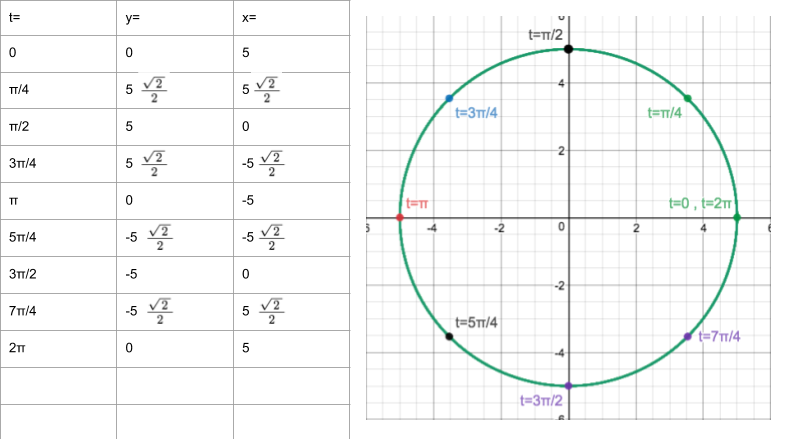
\includegraphics[width = 14 cm, height = 7 cm]{Josh2.png}\\
As you can see the predictions were true. In comparison to the first try it seems much more realistic and smooth.\\\\
\underline{Example Folium}\\
In this section we will be analyzing the graph of the Folium of Descartes. 
First, lets create a table to generalize the points on the graph. Then, we can plot the points and label them showing a path of motion.
\\\\
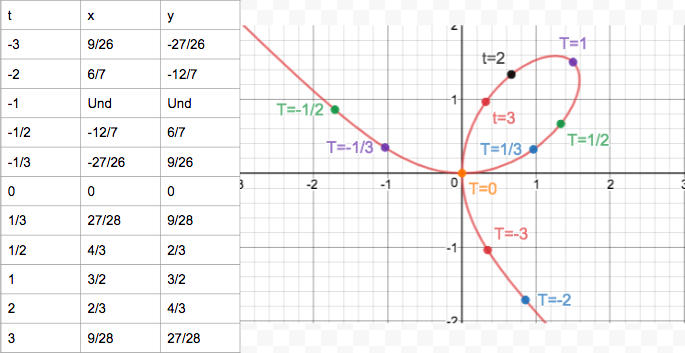
\includegraphics[width = 14 cm, height = 7 cm]{ST.png}


\subsection*{Analysis (points of interest)}
When we talk about the graph we notice how the path of motion is irregular. Now we know that the graph truly begins when $t=0$, however, we shall dive a little deeper and find what happens as $t \rightarrow \infty$ and when $t \rightarrow -\infty$. Lets first set up some limits for the equation of $(\frac{3t}{1+t^3},\frac{3t^2}{(1+t^3)}) $.
$$\lim_{t\to\infty}(\frac{3t}{1+t^3},\frac{3t^2}{(1+t^3)})  $$
We need to use l'hopital's rule in order to crack this one. Using what we know about derivatives we will eventually find that that we are just going to have a "t" in the denominator for both x and y which is just going to make the point $(0,0)$ because as $n/t$, "n" being any number, approaches infinity we are going to end up with a zero. Note that this will be approaching from the top of that starting point.
If we do the same for when $t \rightarrow -\infty$ we will still end up with the same point of $(0,0)$ except it will be approaching from the bottom of the origin. The funny thing is that $t=0$ is the point $(0,0)$
$$\lim_{t\to\infty}(\frac{3t}{1+t^3},\frac{3t^2}{(1+t^3)})  =(0,0)$$\\\\
Now lets see if the graph ends any where, we know that $t=-1$ is undefined yet you get values before and after that. Lets see what happens at we see x(t) and y(t) approaching -1 from both sides.
$$\lim_{t\to\ -1^-} (\frac{3t}{1+t^3},\frac{3t^2}{(1+t^3)}) $$
$$\lim_{t\to\ -1^+} (\frac{3t}{1+t^3},\frac{3t^2}{(1+t^3)}) $$
We cant seem to get anywhere using math so let's try something else. If we look at each component's graph we can start to see the relationship with $t=-1$. \\
\\
First, we'll look at y(t).\\
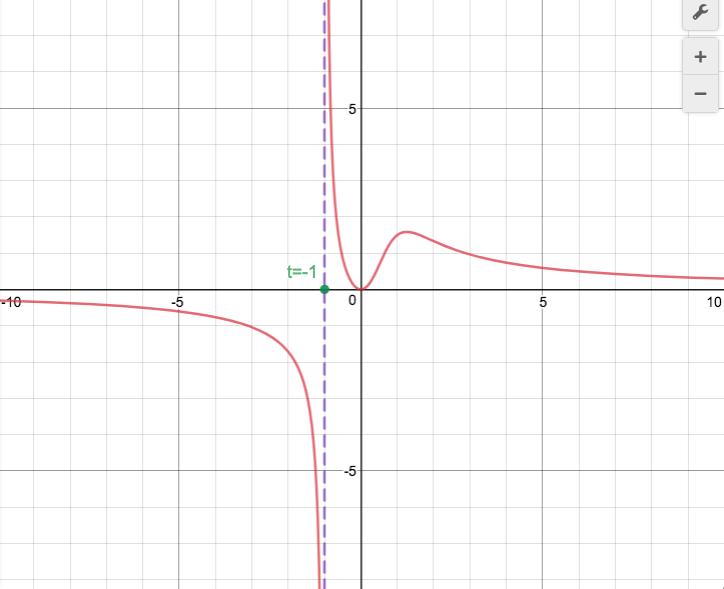
\includegraphics[width = 14 cm, height = 7 cm]{Y(t).png}\\
If we look at the graph, the closer we get to negative side of $t=-1$, y(t) seems to being approaching negative infinity and as we approach from the positive side of $t=-1$, y(t) is going towards positive infinity. Let's use the graph too look at what happens when x(t) approaches from the positive/negative sides of $t=-1$.\\
Graph of x(t).\\
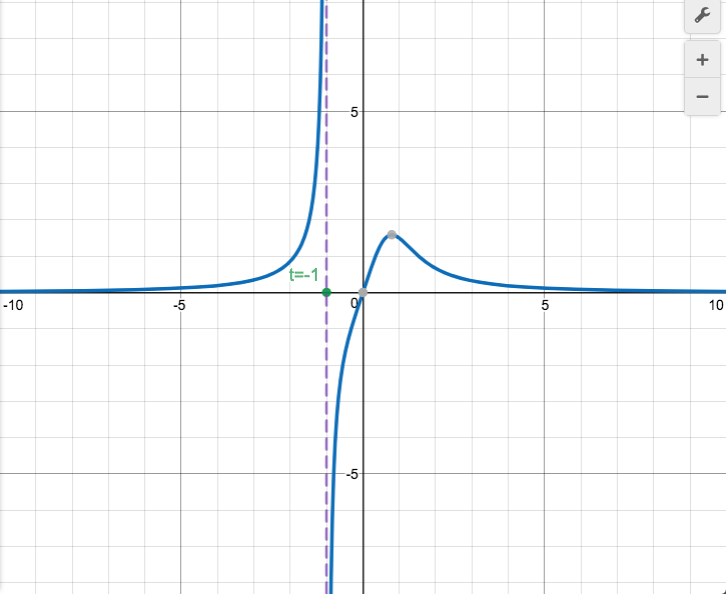
\includegraphics[width = 14 cm, height = 7 cm]{X(t).png}\\
Looking at the graph, the closer we get to negative side of $t=-1$, x(t) seems to being approaching positive infinity and as we approach from the positive side of $t=-1$, x(t) is going towards negative infinity. So, we can say...\\
$$\lim_{t\to\ -1^-} (\frac{3t}{1+t^3},\frac{3t^2}{(1+t^3)})=(\infty,-\infty) $$
$$\lim_{t\to\ -1^+} (\frac{3t}{1+t^3},\frac{3t^2}{(1+t^3)})=(-\infty,\infty) $$
Lets continue our analysis into the specific point that is the tip of the loop. The graph appears to be symmetrical along the line of $y=x$. This means the graph could be an inverse of itself. Lets prove it.We know how a graph becomes its inverse by switching the x and the y value. So let's just do that.
$$x^3 + y^3=3xy$$
Now swap x and y.
$$y^3 + x^3=3yx$$
Since multiplication and addition are both commutative the inverse and the function are still the same thing. This means that we can use the line $y=x$ to find the tip of the loop because you could fold the graph onto itself using the line of $y=x$.\\
\\
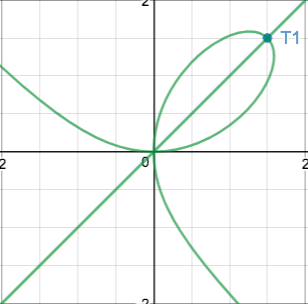
\includegraphics[width = 4 cm, height = 4 cm]{SM.png}\\
With this info we can substitute the $x$ in for $y$ in our folium to find the x-value for the tip. 
$$x^3 + x^3=3x^2$$
$$2x^3=3x^2$$\\
Now lets solve for when for when the equation is equal to 0.
$$2x^3-3x^2=0$$
$$x^2 (2x-3)=0$$
$$x=0,x=3/2$$\\
Now we don't really care for when $x=0$ because when $x=0$,$y=0$ which is just the starting point. So lets just use $x=3/2$ and substitute it into the equation of $y=x$ since it is part of the point of intersection. Once we complete this step, we find that the tip is the coordinate $(3/2,3/2$ which is literally the point in which $t=1$.
\subsection*{Analysis (Tangent Lines)}
-\\

Using the differentiation of parametric equations we can easily discover when there are tangent lines that are vertical, horizontal or at any $t$ value. Let's use the Folium as an example. First lets derive $x(t)$ and $y(t)$ using the rules that we know.
$$x(t)=\frac{3t}{1+t^3}$$\\
$$x'(t)=\frac{-3(2t^3 -1)}{(t^3 +1)^2}$$\\
$$y=\frac{3t^2}{1+t^3}$$\\
$$y'(t)=\frac{-3t(t^3 -2)}{(t^3 +1)^2}$$\\
With these components we can solve for both the horizontal and vertical tangent lines. First let's solve for the horizontal lines. This is going to be the point at which the y coordinate is no longer increasing or decreasing. Since we know the derivative for $y(t)$ we can just set it equal to zero and solve for that t value.
$$y'(t)=0$$\\
$$\frac{-3t(t^3 -2)}{(t^3 +1)^2}=0$$\\
$$t=2^{1/3},t=0$$\\
Now substitute the values in the $y(t)$ and there are your two horizontal tangent lines.
$$y(2^{1/3})=\frac{3(2^{1/3})^2}{1+(2^{1/3})^3}=2^{2/3}$$\\
$$y(0)=\frac{3(0)^2}{1+(0)^3}=0$$\\
So $y=0$ and $y=2^{2/3}$ are the two tangent lines.\\\\
Now lets solve for the vertical lines. Same process and thinking except with x values. This time we are going to solve when $x'(t)=0$.
$$x'(t)=0$$\\
$$\frac{-3(2t^3 -1)}{(t^3 +1)^2}=0$$\\
$$t=\frac{1}{2^{1/3}}$$\\
Substitute into $x(t)$
$$x(\frac{1}{2^{1/3}})=\frac{3(\frac{1}{2^{1/3}})^2}{1+(\frac{1}{2^{1/3}})^3}=2^{2/3}$$\\
So the vertical line is just going to be at $x=2^{2/3}$.\\

Lastly we need to find the tangent line of the tip. We know that the $t$ value is going to be 1. We also can figure out the slope of the tangent line using the idea that $dy/dx$ is just equal to $\frac{dy/dt}{dx/dt}$ because it is the slope of the both rates moving along the xy plane. So let's start.
$$\frac{dy}{dx}=\frac{y'(t)}{x'(t)}$$
$$\frac{dy}{dx}=\frac{\frac{-3t(t^3 -2)}{(t^3 +1)^2}}{\frac{-3(2t^3 -1)}{(t^3 +1)^2}}$$
$$\frac{dy}{dx}=\frac{t(2-t^3)}{1-2t^3}$$
Now substitute in 1.
$$\frac{dy}{dx}=\frac{1(2-(1)^3)}{1-2(1)^3}=-1$$
Now put slope into equation. Use slope intercept form with the values of $x=3/2$ and $y=3/2$ because this is a point that will be on our line.
$$y=-(x-3/2)+3/2$$

One more thing with tangent lines, we can find the equation of the asymptote using them. First, we know that the graph is undefined at the t value of -1. Also when the graph is approaching the asymptote the its is approaching from both sides to the coordinate of which t=-1. So substitute this value into our first derivative.
$$\frac{dy}{dx}=\frac{-1(2-(-1)^3)}{1-2(-1)^3}=\frac{-3}{3}=-1$$
Now that we have have the slope all we need is a point along the line in order to find the intercept. Lets used the implicit differentiated version of the derivative which would be in terms of x and y.
$$x^3 + y^3=3xy$$
Implicit differentiation
$$3x^2+3y^2 \frac{dy}{dx} =3x\frac{dy}{dx} + 3y$$
$$\frac{dy}{dx}=\frac{y-x^2}{y^2 - x}$$
We know that the slope is $-1$, so lets set $-1=\frac{dy}{dx}$ and use the idea about finding a point on the line to find a specific solution. The easiest point to solve for would be an x or y intercept because that is when x or y is equal to zero and other coordinate is some value. So in the differential equation substitute zero in for x or y and solve for the other knowing that $-1=\frac{dy}{dx}$. I will be setting $x=0$.
$$-1=\frac{y-x^2}{y^2 - x}$$
$$-1=\frac{y-0^2}{y^2 - 0}$$
$$-1=\frac{y}{y^2}$$
Simplify.
$$-1=\frac{1}{y}$$
Now multiply $-y$ to both sides.
$$-y(-1=\frac{1}{y})$$
$$y=-1$$
Now that we have why our intercept and slope we can write an equation for the tangent line.
$$y=-x-1$$
\\
Now the whole graph with all the tangents lines and the asymptote will be below.\\

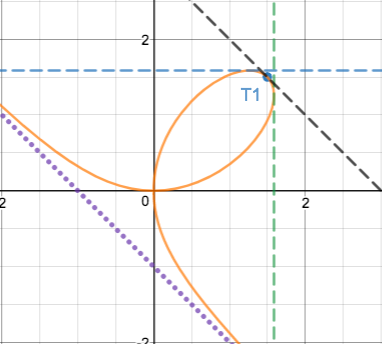
\includegraphics[width = 10 cm, height = 10 cm]{FG.png}
\\*Folium with asymptote and tangent lines.



 \section*{First and Second Derivatives}
 Derivatives of parametric equations are very similar to other derivatives. It starts like any other derivative with $\frac{dy}{dx}$ which is the common equation for a derivative showing the change in y over the change in x demonstrated by this graph, 
 \begin{center}
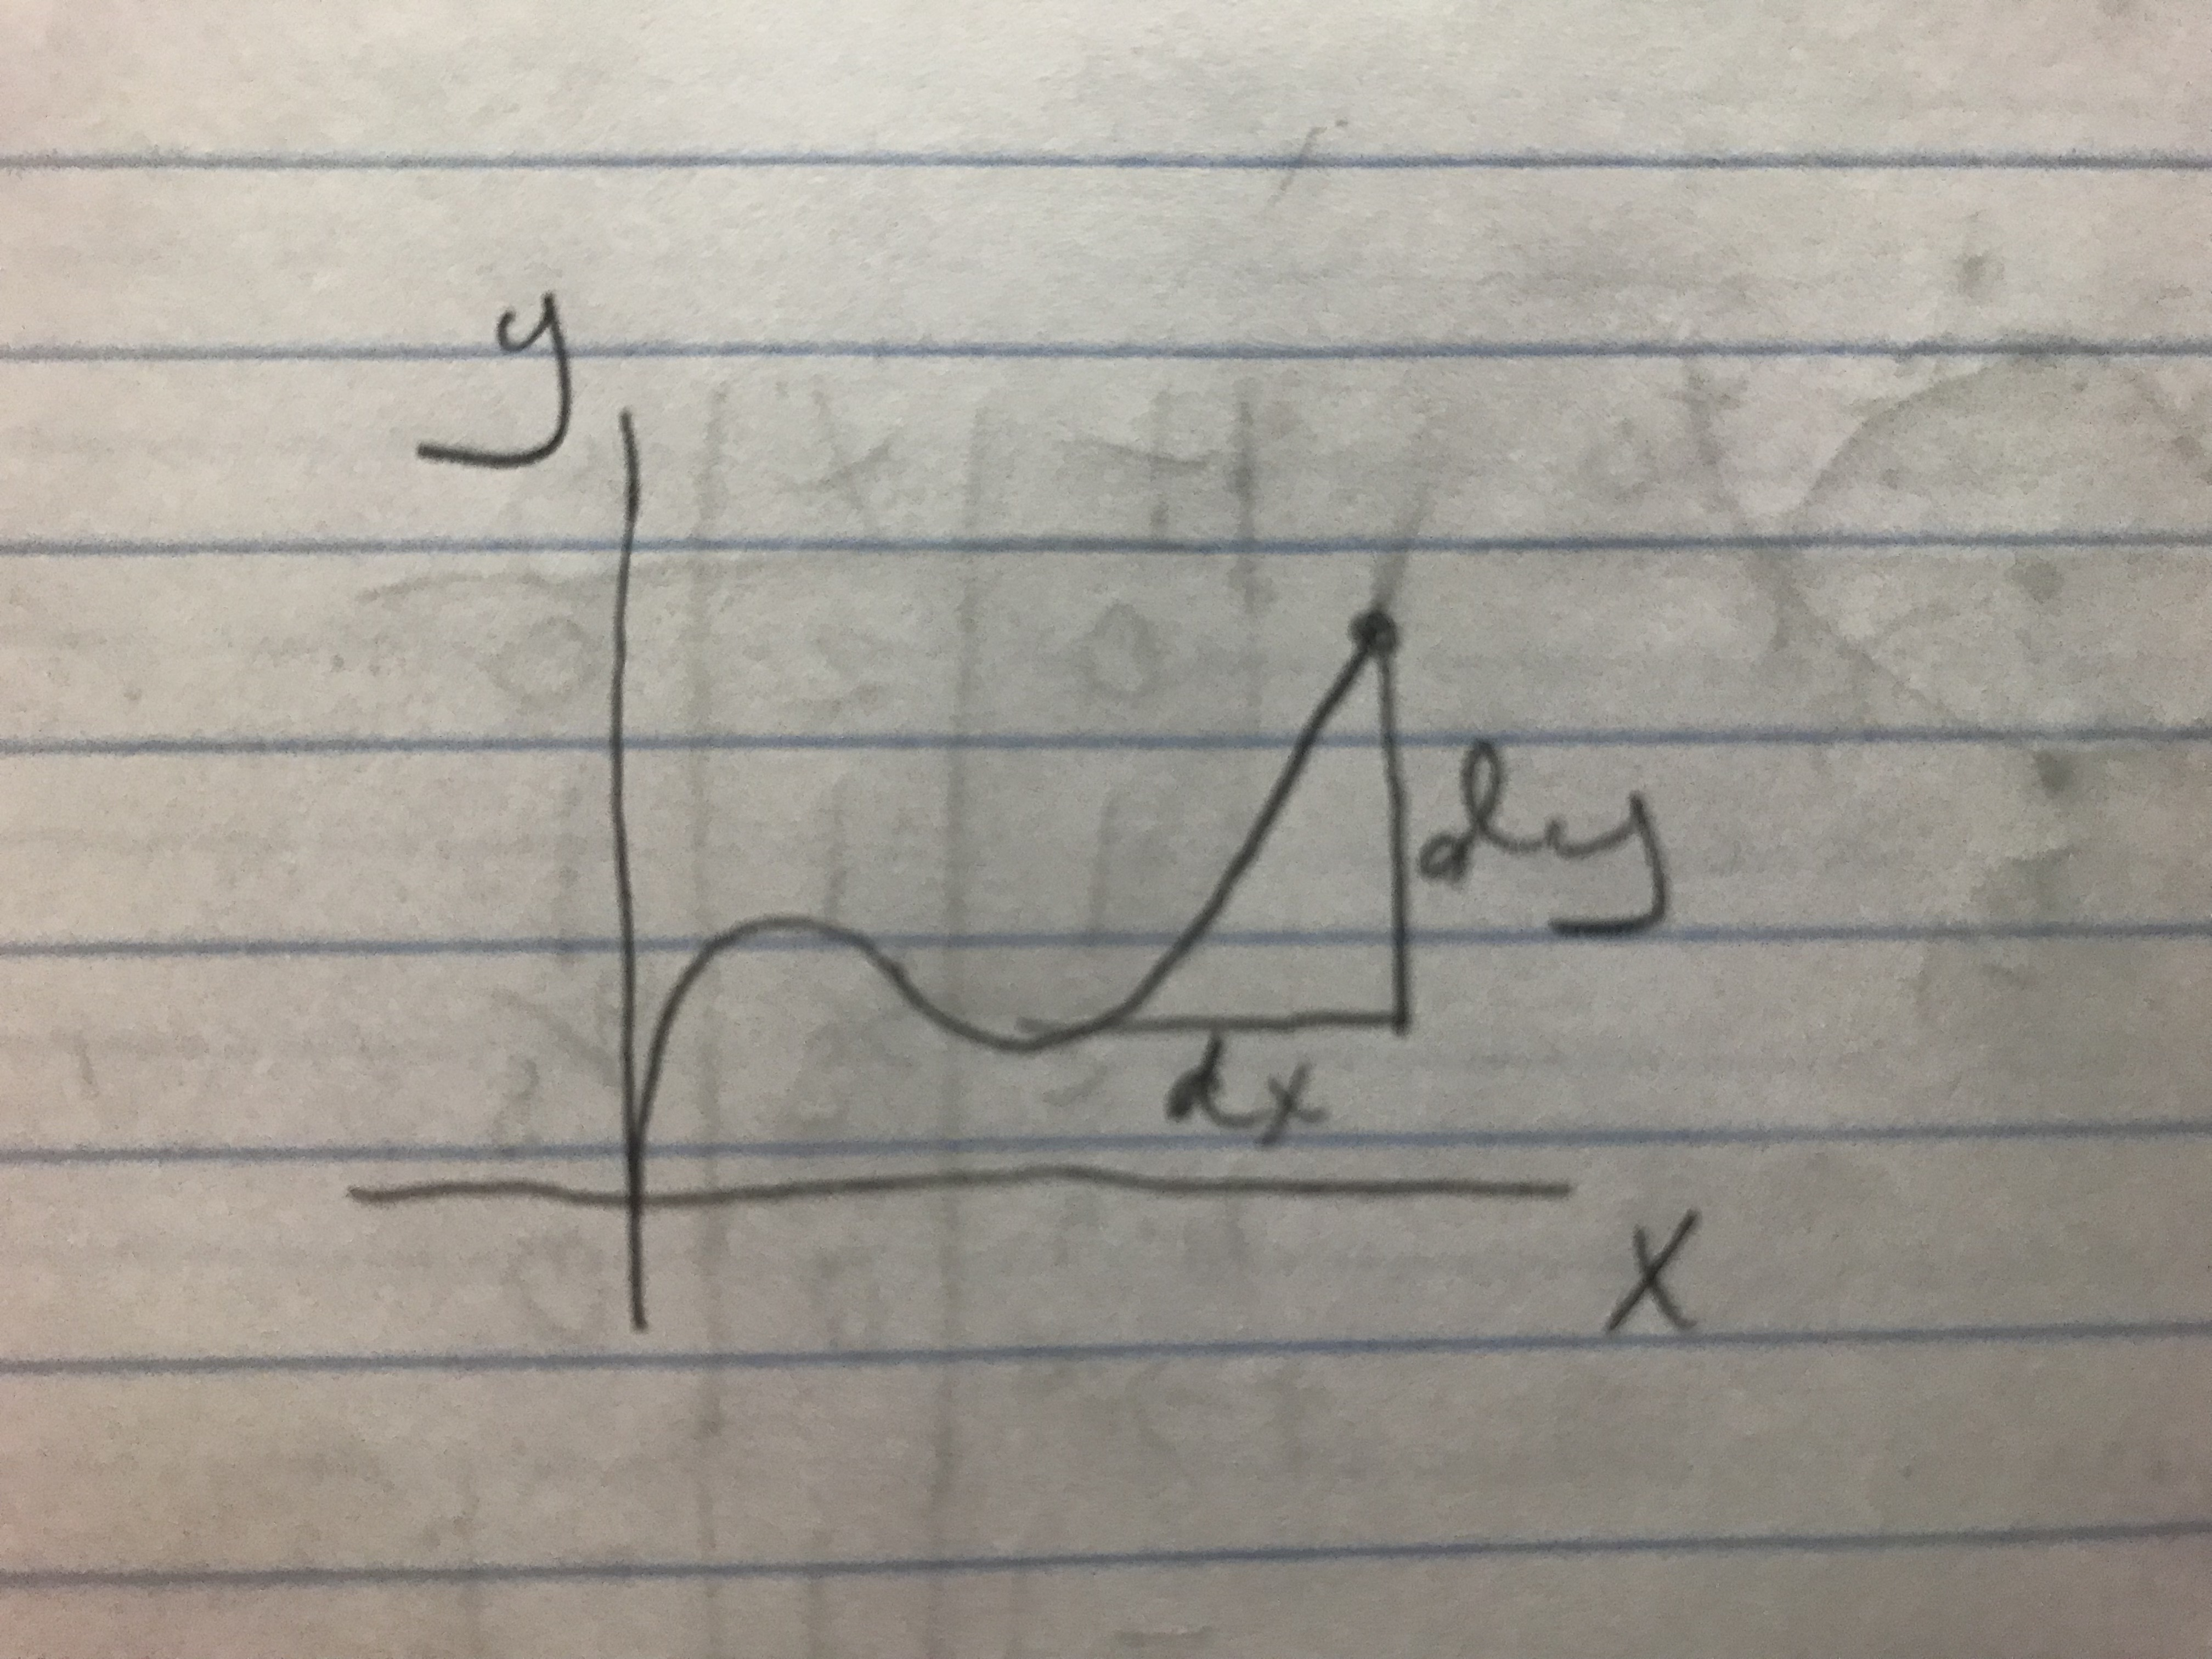
\includegraphics[width = 10 cm, height = 7 cm]{graph.JPG}
\end{center}but parametric equations are in terms of t and since the normal derivative takes the derivative of y and divides it by the derivative of x we can do the same thing with the parametric equations using their components. The derivatives of each component are just in terms of t so for the the y component the derivative is $\frac{dy}{dt}$  and the x component is $\frac{dx}{dt}$. With these we can make the equation of 
 $$\frac{dy}{dx}=\frac{\frac{dy}{dt}}{\frac{dx}{dt}}$$
 To find the second derivative of the equation we have to find the derivative of the original derivative making $$\frac{dy^2}{d^2x}=\frac{d}{dx}(\frac{dy}{dx})$$ a graph of this would look like this  \begin{center}
    

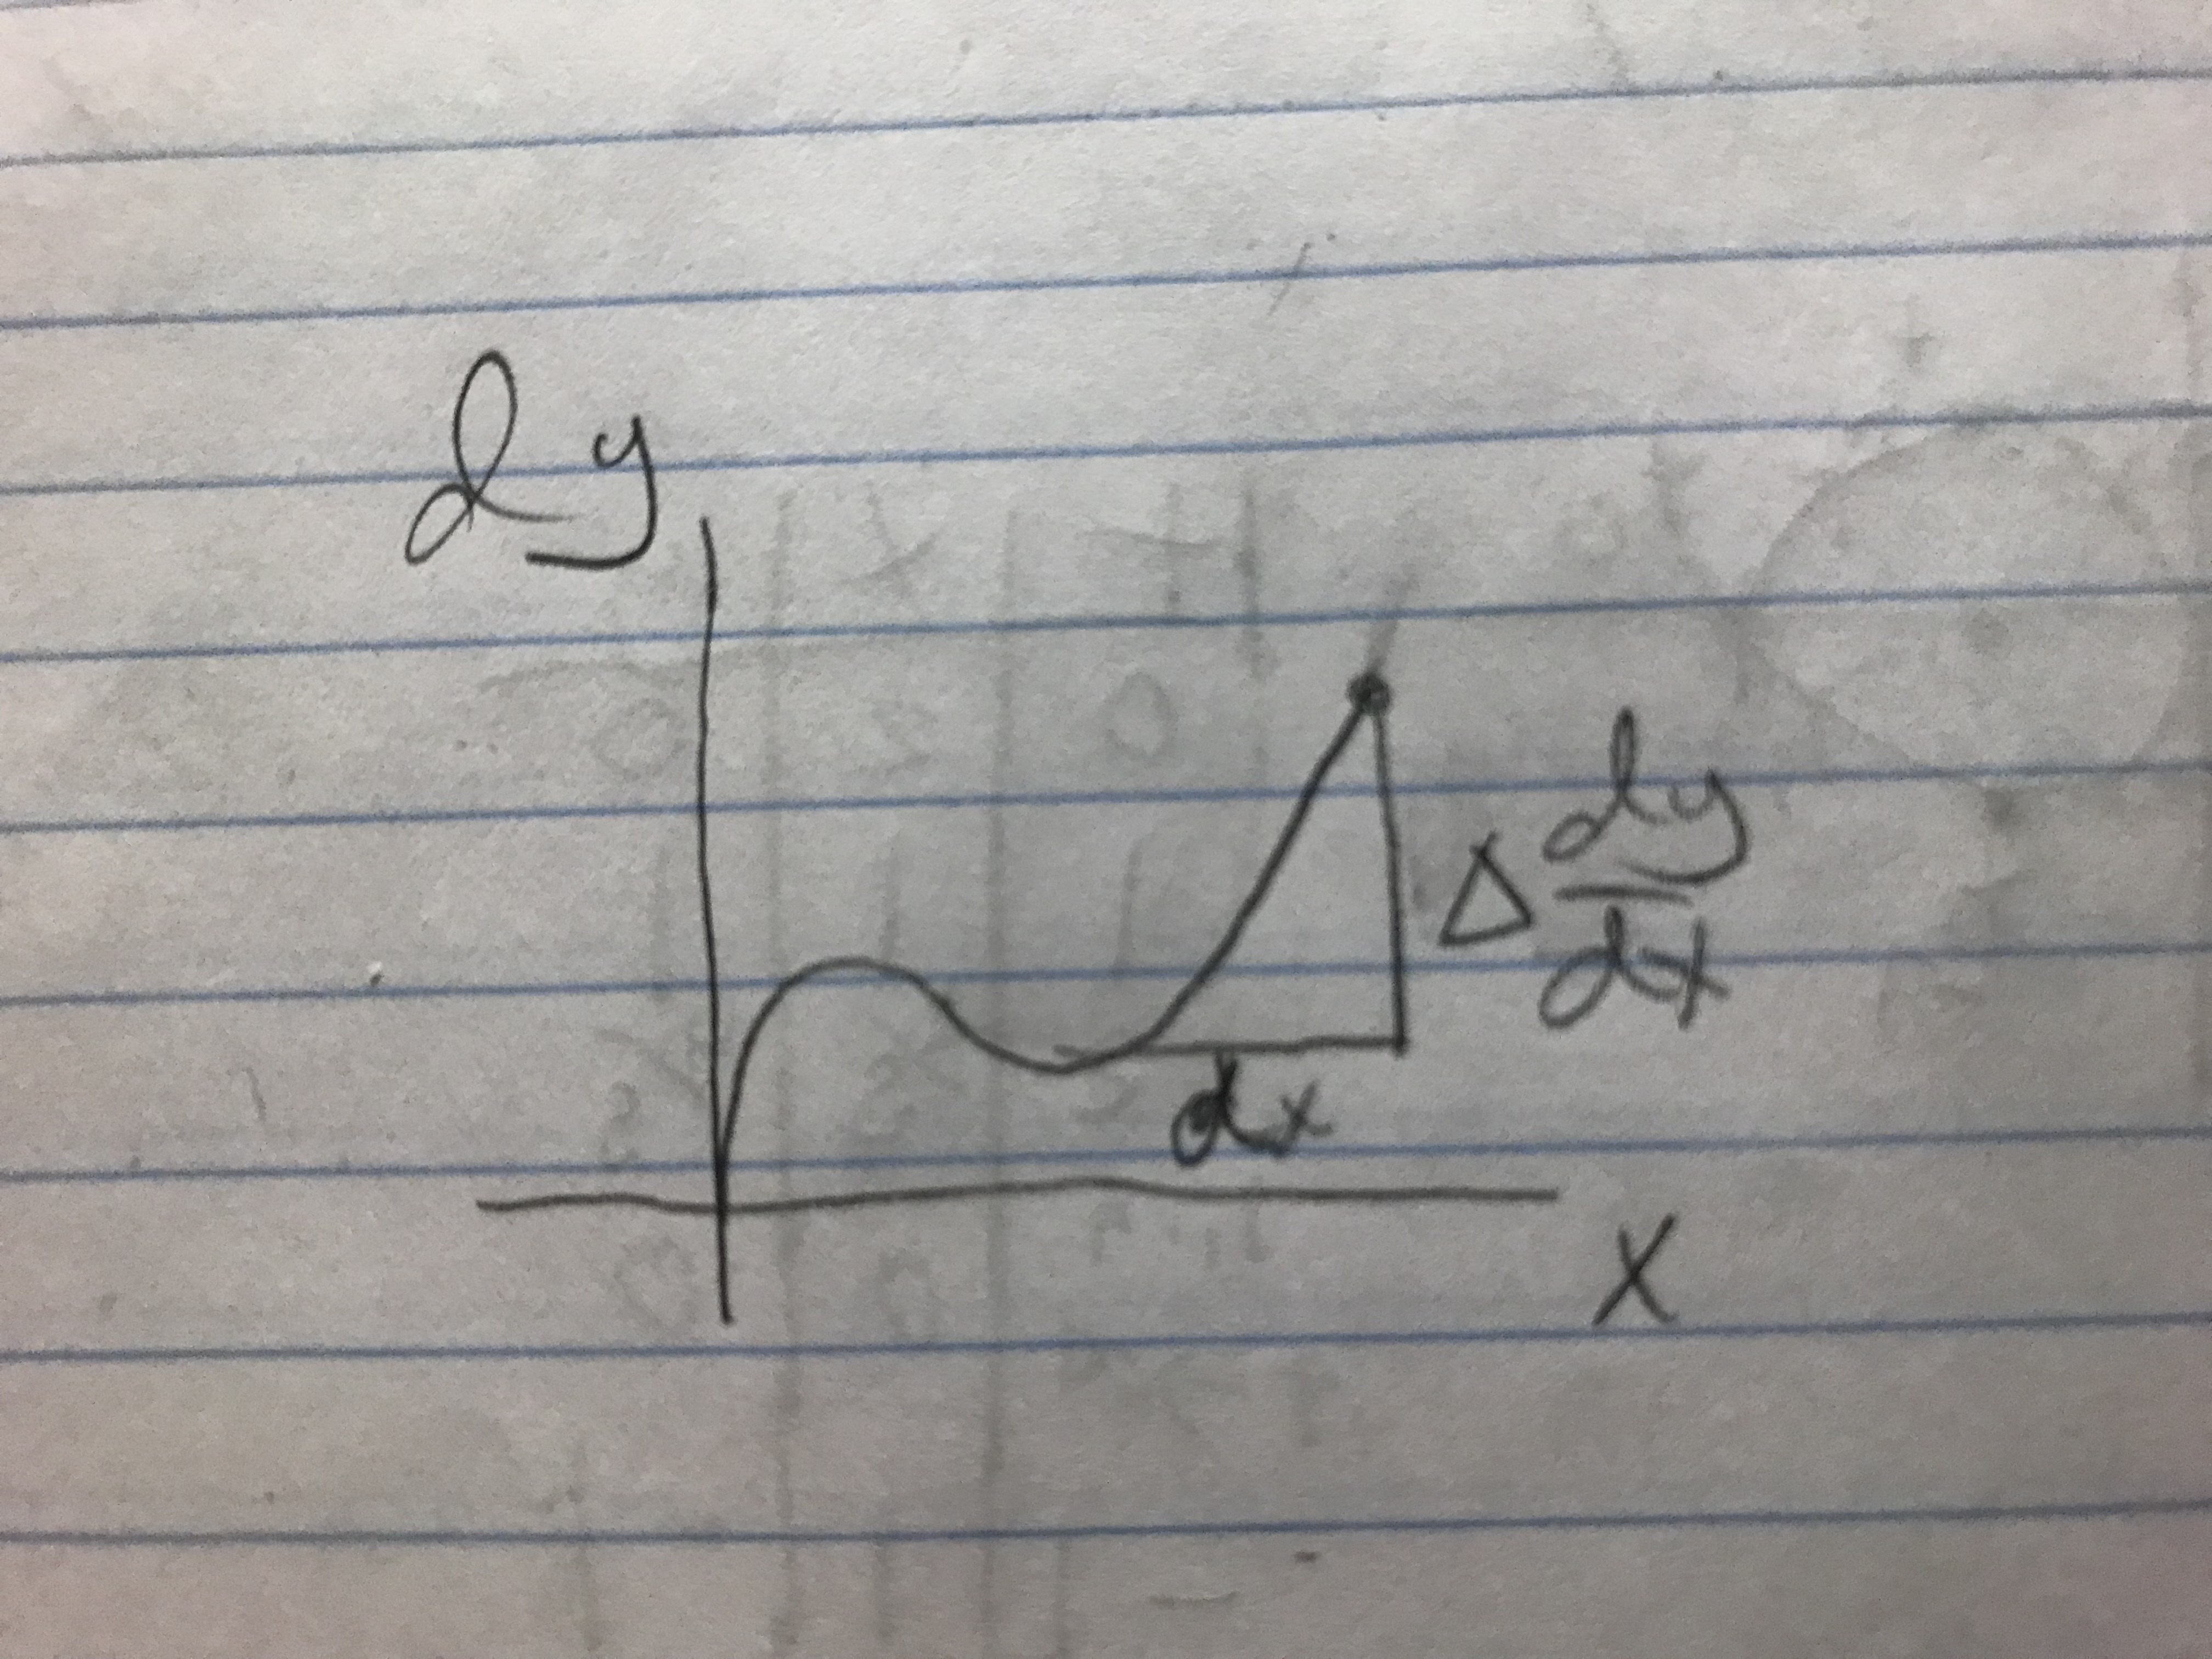
\includegraphics[width = 10 cm, height = 7 cm]{christmas.JPG}
\end{center}
Then when the equation is put into in parametric form and taken with respect to t it turns the equation into this  $$\frac{dy^2}{d^2x}=\frac{\frac{d}{dt}}{\frac{dx}{dt}}({\frac{dy}{dx}})$$ which makes 
 $$\frac{dy^2}{d^2x}=\frac{\frac{d}{dt}(\frac{dy}{dx})}{\frac{dx}{dt}}$$
 Examples:\\\\
 \underline{Example 1} Find the second derivative of the parametric equations $y=17t^3-6t^2$ and $x=\frac{3t}{2}$\\\\
 First we start by finding the first derivative which we found is just the derivative of the y portion divided by the derivative of the x portion which is $$\frac{51t^2-12t}{\frac{3}{2}}$$ which equals $$\frac{102t^2-24t}{3}$$ and then to find the second derivative we have to take the derivative of the piece that we just found which is $$\frac{204}{3}t-\frac{24}{3}$$ and when put into the equation of the second derivative we get $$\frac{dy^2}{d^2x}=\frac{\frac{204}{3}t-\frac{24}{3}}{\frac{3}{2}}$$ which simplifies to $$\frac{dy^2}{d^2x}=\frac{136t-16}{3}$$
 \underline{Example 2}
 Find the second derivative of $x=e^{-t}$ and $y=e^t$.
\\\\We start this one like the last one, by finding the derivatives. The derivative of the x component is $-e^{-t}$ and the derivative of the y component is $e^t$, so $$\frac{dy}{dx}=\frac{e^t}{-e^{=t}}$$ just simplifies to $$\frac{dy}{dx}=-e^{2t}$$
To find the second derivative we take the derivative of this and divide it by the derivative of the x portion. The derivative of $\frac{dy}{dx}$ however is just $-2e^2t$ which means that $$\frac{dy^2}{d^2x}=\frac{=2e^2t}{-e^{-t}}$$ which can be simplified down to $$\frac{dy^2}{d^2x}=2e^{3t}$$
\underline{Example 3} Find the second derivative of an equation where the parametric equations are $x=2cost$ and $y=2sint$ the derivatives are these are $$\frac{dy}{dt}=2cost$$ and $$\frac{dx}{dt}=-2sint$$ and that means $$\frac{dy}{dx}=\frac{2cost}{-2sint}$$ or $-cott$ and when we take the derivative of that we get $$(csct)^2$$ and then we can substitute that into the second derivative equation making $$\frac{dy^2}{d^2x}=\frac{(csct)^2}{-2sint}$$
\underline{Example 4}
Find the second derivative of the parametric equations $x=t^2$ and $y=t^3$ the derivatives of these are $\frac{dx}{dt}=2t$ and $\frac{dy}{dt}=3t^2$ so that means that $$\frac{dy}{dx}=\frac{3t^2}{2t}$$ this simplifies down to $$\frac{dy}{dx}=\frac{3t}{2}$$ but it has to be mentioned that t cannot equal 0 as it makes the denominator 0 before it is simplified.
We have to derive again to find the second derivative which makes $\frac{3}{2}$ and the we can substitute that in making $$\frac{dy^2}{d^2x}=\frac{\frac{3}{2}}{2t}$$ which simplifies down to $$\frac{dy^2}{d^2x}=\frac{3}{4t}$$
\section*{Tangent Lines}
We can use our knowledge of parametric derivatives to help us find horizontal and vertical tangent lines for parametric equations. Let's use the knowledge that 
$$\frac{dy}{dx}=\frac{\frac{dy}{dt}}{\frac{dx}{dt}}$$ to find when a horizontal or vertical tangent line exists.\\\\
A horizontal tangent line exists when the numerator of $\frac{dy}{dx}$ is 0 and the denominator is a non-zero number. If we use our past knowledge, this would make sense because it would mean that $\frac{dy}{dt}$, which is in the numerator, would have to equal 0. If we think about the way a horizontal line moves, the x values are changing, but there would be no change in y values, proving that the change in y over time, or $\frac{dy}{dt}$ would be 0. Let's look at the graph of a horizontal line below so we can visualize this.
\begin{center}
    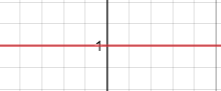
\includegraphics[width= 5cm, height=3cm]{Images/horizline.png}
\end{center}
A vertical tangent line exists when the denominator of $\frac{dy}{dx}$ is 0 and the numerator is a non-zero number. If we use our past knowledge, this would make sense because it would mean that $\frac{dx}{dt}$, which is in the denominator, would have to equal 0. If we think about the way a vertical line moves, the y values are changing, but there would be no change in x values, proving that the change in x over time, or $\frac{dx}{dt}$ would be 0. Let's look at the graph of a vertical line below so we can visualize this.
\begin{center}
    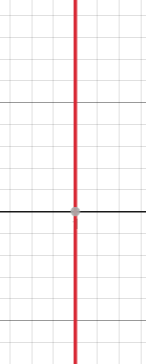
\includegraphics[width=3cm, height=5cm]{Images/vertline.png}
\end{center}
A break or corner on the graph exists when both $\frac{dy}{dt}$ and $\frac{dx}{dt}$ equal zero. This would mean that $\frac{dy}{dx}$ would equal $\frac{0}{0}$ which is non-real and cannot exist. Therefore, it would make sense that this indicates where a corner or break is, since we can’t take the derivative there. 
\\\\
Examples:\\
\underline{Example 1}
Identify any tangent lines in the parametric curve given by:
$$y=\frac{2}{3}t^3-\frac{1}{2}t^2$$
$$x=\frac{1}{2}t^2-3t$$
First we’ll want to find $\frac{dy}{dt}$ and $\frac{dx}{dt}$.
$$\frac{dy}{dt}=2t^2-t$$
$$\frac{dx}{dt}=t-3$$
Now we’ll use our knowledge that $\frac{dy}{dx}=\frac{\frac{dy}{dt}}{\frac{dx}{dt}}$
$$\frac{dy}{dx}=\frac{2t^2-t}{t-3}$$
Factor the numerator.
$$\frac{dy}{dx}=\frac{t(2t-1)}{t-3}$$
Set the numerator equal to zero to find when $\frac{dy}{dt}=0$, or the horizontal tangent lines.
$$t(2t-1)=0$$
$$2t-1=0$$
$$t=\frac{1}{2}$$
$$t=0$$
So, we know that there are horizontal tangent lines at $t=0$ and $t=\frac{1}{2}$.\\
Now let’s set the denominator equal to 0 to find the vertical tangent lines.
$$t-3=0$$
$$t=3$$
We know that there’s a vertical tangent line at $t=3$. Let’s look at the graph of the parametric with its tangent lines drawn in to show that this is true.
\begin{center}
    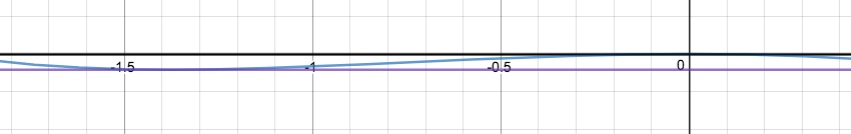
\includegraphics[height=5cm, width=8cm]{Images/tangent.png}
\end{center}
We can see in this image that the horizontal lines on the top and bottom of the graph that touch the graph at a point are the horizontal tangent lines.
\begin{center}
    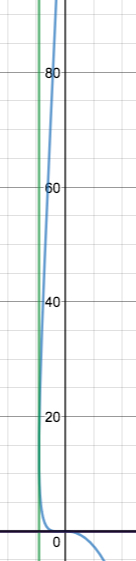
\includegraphics[height=8cm, width=4cm]{Images/tangentline.png}
\end{center}
We can see in this image that the vertical line on the left of the graph that touches the graph at a point is the vertical tangent line.\\\\
\underline{Example 2}
Identify any tangent lines in the graph over the interval $0\leq t\leq \pi$ given by:
$$y=sin(2t)$$
$$x=-cos(2t)$$
Find $\frac{dy}{dt}$ and $\frac{dx}{dt}$.
$$\frac{dy}{dt}=2cos(2t)$$
$$\frac{dx}{dt}=2sin(2t)$$
Write $\frac{dy}{dx}$.
$$\frac{dy}{dx}=\frac{2cos(2t)}{2sin(2t)}$$
To find the horizontal tangent lines, set the numerator equal to 0. 
$$2cos(2t)=0$$
$$cos(2t)=0$$
$$t=\frac{\pi}{4}$$
$$t=\frac{3\pi}{4}$$
Now, we know that there are horizontal tangent lines where $t=\frac{\pi}{4}$ and $t=\frac{3\pi}{4}$.\\\\
To find the vertical tangent lines, set the denominator equal to 0.
$$2sin(2t)=0$$
$$sin(2t)=0$$
$$t=\frac{\pi}{2}$$
$$t=\pi$$
Now, we know that there are vertical tangent lines at $t=\frac{\pi}{2}$ and $t=\pi$. Let’s look at the graph of the parametric with its tangent lines drawn in to show that this is true.
\begin{center}
    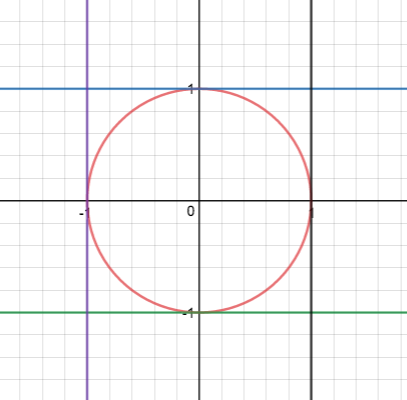
\includegraphics[height=4cm, width=4cm]{Images/circletan.png}
\end{center}
\underline{Example 3}
Identify the break in the parametric equation given by:
$$y=4t^2+1$$
$$x=3t^2-2$$
Find $\frac{dy}{dt}$ and $\frac{dx}{dt}$.
$$\frac{dy}{dt}=8t$$
$$\frac{dx}{dt}=6t$$
Rewrite $\frac{dy}{dx}$.
$$\frac{dy}{dx}=\frac{8t}{6t}$$
We can see that both the numerator and denominator would equal 0 when $t=0$. Therefore, there is a break in the graph at $t=0$. 
\ssection{Polar Equations}
\section*{Introduction}
Polar form is a different form of expressing rectangular coordinates that allows us to easily create unique shapes such as circles. Polar form is written differently from rectangular form, but with some practice, it can be easily interpreted and complex shapes such as limacons can be drawn. We can also use derivatives to find the equation of the tangent line on a polar graph. We can also find the area of a polar graph and even find the area between two polar curves. Let’s start off by exploring the different types of polar shapes.
\section*{Lines - Circles - Limacons - Lemniscates - Polar Roses - Spirals} These shapes are built and formed with polar equations. Polar equations use radius and angle instead of x and y to plot coordinates.
\\Lines are formed by a degree of theta, which is an angle. It can be written as just an angle or the form of $$\theta=tan^{-1}(a)$$
an example is $$\theta=tan^{-1}(\sqrt{3})$$ which looks like this 
\begin{center}
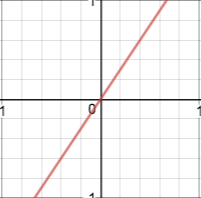
\includegraphics[width = 5 cm, height = 5 cm]{line.png}
\end{center}
\\polar circles are formed by the equation $r=asin\theta$ and $r=acos\theta$ and can also be formed with the equation $r=a$ because all it is, is just a radius take the equation of $r=2cos(\theta)$ which looks like this \begin{center}
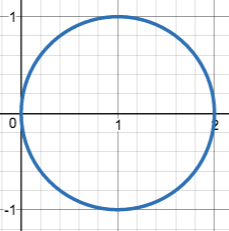
\includegraphics[width = 5 cm, height = 5 cm]{circle.png}
\end{center}
we see that a determines the diameter of the circle and that it is made off center on the x axis, the sin graph would be shifted 90 degrees on to the y-axis and the equation that doesn't have trig in it will from a circle at the origin with a being the radii instead of the diameter. Any negative graph would just rotate each graph 180 degrees. With the cos graph it start at (0,2) and moves counterclockwise around the circle and the sin graph will start at 0 and will move around the same way
There are multiple forms of limacons such as: ones with an inner loop, dimpled, convex and in some cases cardioids. These are all formed by the equation $$r=a\pm bcos(\theta)$$ or $$r=a\pm bsin(\theta)$$ 
It all depends on the ratio of a to b to determine the shape. However, this ratio is always positive and absolute value is used. If $a=b$ then the shape formed is a cardioid. If $a:b<1$ than the shape formed is a limacon with an inner loop. If $1<a:b<2$, then a dimpled limacon is formed. This is different from a cardioid because the dimple doesn't touch the origin, while a point on the cardioid does touch the origin. If $a:b\geq2$ a convex limacon is formed which looks like a circle, but isn't because one side is slightly flatter than the other. These are the cosine versions of all of their graphs
\begin{center}
    
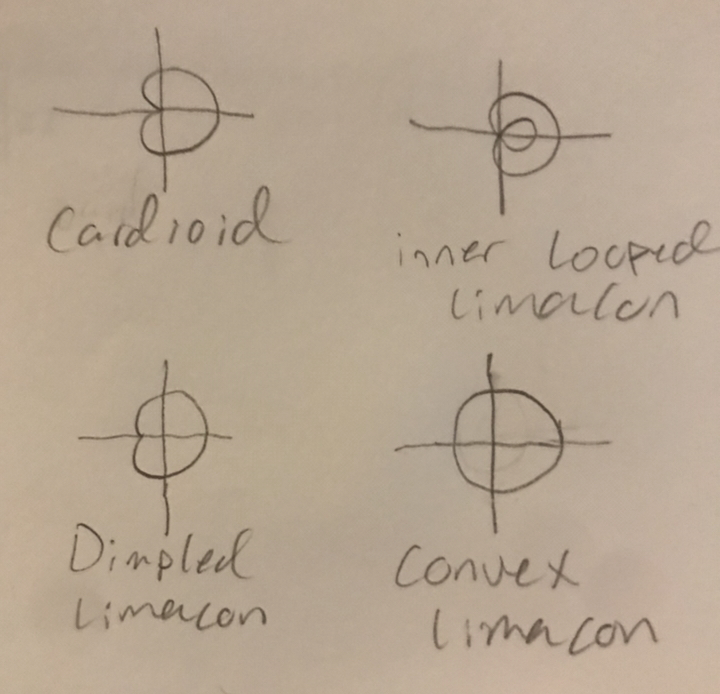
\includegraphics[width = 10 cm, height = 10cm]{graphs.jpg}
\end{center}
The sine graphs would look the same, just rotated 90 degrees counterclockwise. If b is negative, then either graph would be rotated 180 degrees. The cosine graphs start at 0 and then a distance on the x axis relative to a while the sin graphs start at (0,0) and both of them move counterclockwise.
\\Lemniscates are formed from the equation $r^2=a^2sin(2\theta)$ or $r^2=a^2cos(2\theta)$ an example is when $a=4$ and we square root both sides making $r=\pm \sqrt{16sin(2\theta}$ which looks like this \begin{center}
    

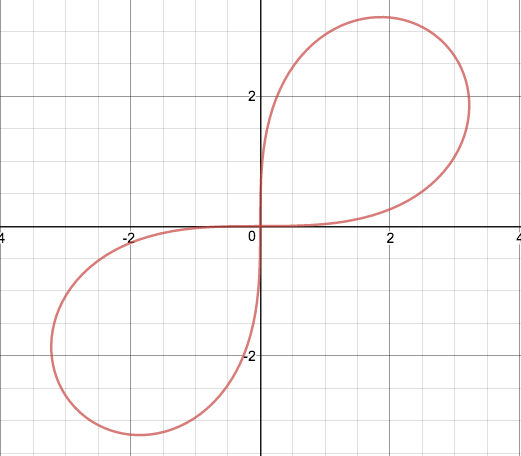
\includegraphics[width = 5 cm, height = 4cm]{sin.png}
\end{center}and both the positive and negative have the same graph because of the square root eliminating any negative that are formed by using second and fourth quadrant points. The sin graph starts from (0,0) and goes counterclockwise. If you used cosine it would look like this \begin{center}
    

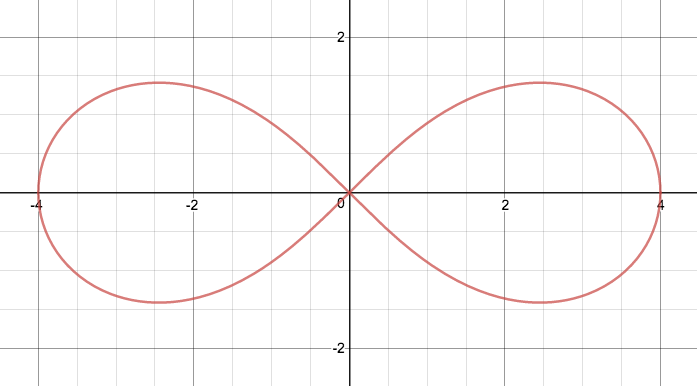
\includegraphics[width = 5 cm, height = 3.5 cm]{cos.png}
\end{center}
The cos graph starts from $(0,\sqrt{a})$ and goes counterclockwise. It doesn't go around like how an eight is drawn it goes through the quadrants in order so it builds half of the 2 parts at a time.
\\
\\Polar roses are easy to remember to remember what they look like because they have petals like a flower. Rose curves come from the equation $r=asin(n\theta)$ or $r=acos(n\theta)$ and a and n are not equal to 0. n focuses on shape and a focuses on radius. 
\\whatever gets substituted in for n
can make all kinds of patterns like a Spirograph like this one of the graph $r=2sin(.4\theta)$ which looks like this
\begin{center}
    

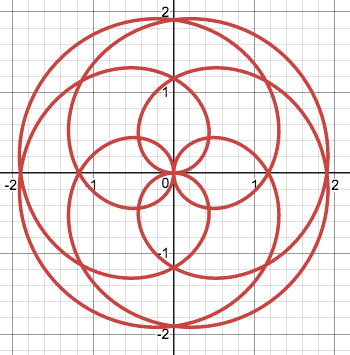
\includegraphics[width = 5 cm, height = 5 cm]{shape.png}
\end{center}
The main focus however is on integers which actually have the petals. The a just defines the radius of the graph like if it was 2 it would go 2 in all directions. The n value is really what decides the shape. if the n is even then there is 2n petals and if n is odd than there is n petals. In the graph of $r=2cos(8\theta)$ which looks like this \begin{center}
    

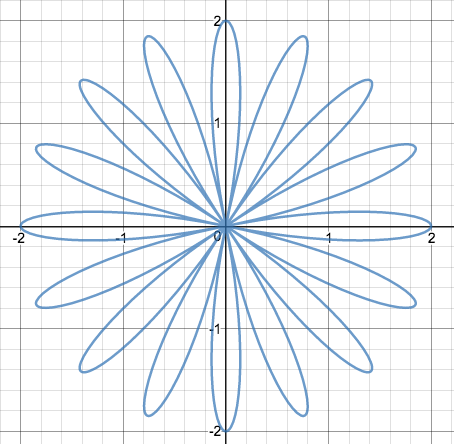
\includegraphics[width = 5 cm, height = 5 cm]{shapes.png}
\end{center} we see that it has 16 petals and because it is a cos graph it starts at (0,a) and the sin graph would be shifted clockwise and starts at (0,0) 
a graph of an equation of an odd n with the equation $r=2sin(5\theta)$ looks like this \begin{center}
    

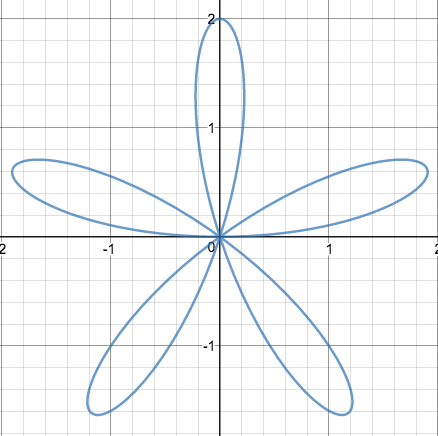
\includegraphics[width = 5 cm, height = 5 cm]{shapes2.png}
\end{center}
we see that this one has 5 petals because n=5 which is odd. The cos graph would just be shifted clockwise 90 degrees. If any of the graphs would be negative then their graphs would be rotated 180 degrees
\\Polar spirals are what you would expect, a spiral. they are formed by the equation $r=n\theta$ and the spiral's  length is dictated by the bounds of the graph. Here is a graph of a spiral with the equation $r=2\theta$ over the interval $0 \leq \theta \leq 2\pi$
\begin{center}
    

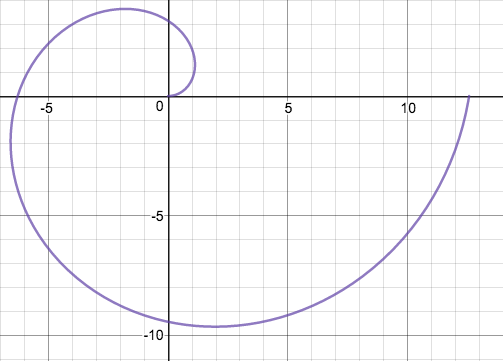
\includegraphics[width = 7 cm, height = 5 cm]{spiral.png} 
\end{center}
It's not much a spiral now because it is from $0 \leq \theta \leq 2\pi$ which makes only one rotation from 0 counterclockwise until it makes one rotation. Then in the graph of the negative $r=-2\theta$ it is rotated 180 degrees. 
\begin{center}
    

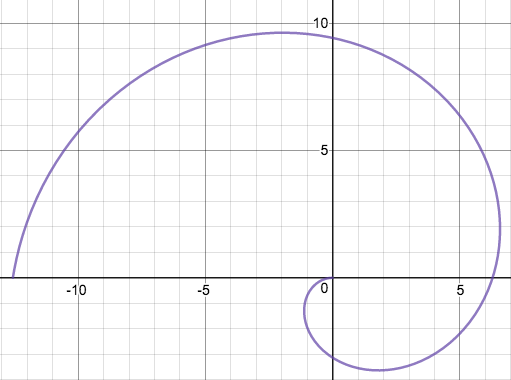
\includegraphics[width = 7 cm, height = 5 cm]{negspiral.png}
\end{center}
\\In the next picture we see a actual spiral because it is the same graph of $r=2\theta$ but it is over the interval $0 \leq \theta \leq 4\pi$ 
\begin{center}
    

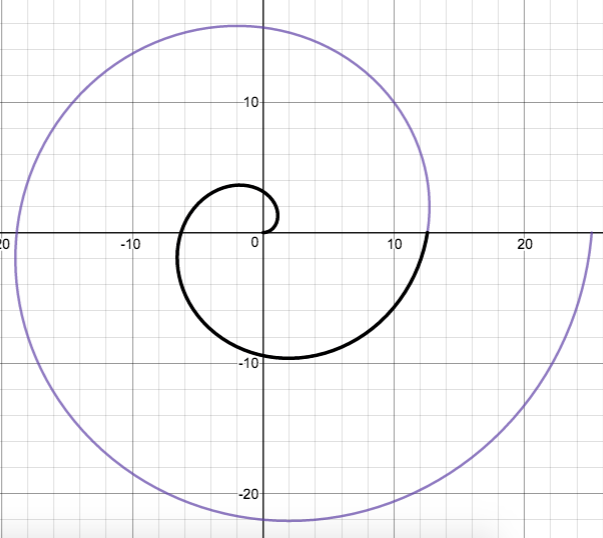
\includegraphics[width = 5.5 cm, height = 5 cm]{bigspiral.png}
\end{center}
we can see two full rotations in this image with each starting from the x axis and going around in a circle and then every consecutive rotation continues from the first rotation.
\\we now know what all the graphs look like, and we know that cos and sin graphs are the same, but shifted and that any graph that is negative will be shifted 180 degrees and that sin will always be 0 when theta is 0 and cos can have any of the a values when theta is 0. 
\\Here are some examples of the graphs.\\
\\\underline{Example 1}
What does this equation look like as a graph? $r=2-2sin\theta$
We can use what we just learned knowing that the only graph with multiple pieces is a limacon and we also see that a and b will be the same so it is in fact a cardioid. another way you can find out what it looks like is by substituting in values for theta around the unit circle. We know what a cardioid looks like, but we can determine it's place from knowing that it is a sin graph so it will fall on the y-axis and since it is negative in one place the graph will be on the negative side of the origin on the y-axis so it will look like this \begin{center}
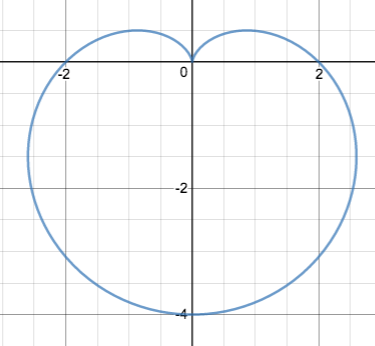
\includegraphics[width = 5.5 cm, height = 5 cm]{ALEX1.png}
\end{center}\\
\\\underline{Example 2}
What does this equation look like as a graph? $r=\sqrt{4cos(2\theta)}$ This one is as you probably guessed a lemniscate because it has not just a multiplied theta, but also it has a square root which shows that it is definitely a lemniscate. and since it is cos we know that it is along the x-axis so it must look like this  \begin{center}
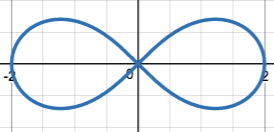
\includegraphics[width = 8 cm, height = 5 cm]{ALEX2.png}
\end{center}
and since it is a cos graph it starts at (0,2)
\\\underline{Example 3}
What does this equation look like as a graph? $r=3sin4\theta$ 
First of all we know it is a polar rose because theta is multiplied by a number and it is not a lemniscate. We know it will have 8 petals because n is 4 which is even and because it is a sin graph we know that it won't hit an axis in the middle of any petals so that means we divide the petals between the 4 quadrants making two petals for each quadrant, so it should look a little something like this 
\begin{center}
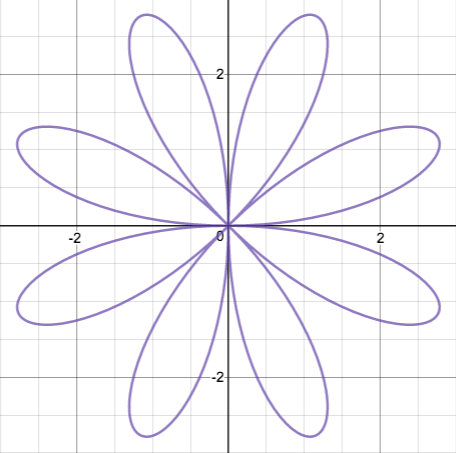
\includegraphics[width = 5 cm, height = 5 cm]{ALEX3.png}
\end{center}
\\\underline{Example 4}
What does this equation look like as a graph? $r=-4sin\theta$ Well we know that it has a number times a trig function which makes it a circle and the sin means that it will be on the y axis and sing it is negative it will be in the lower half of the plane and since it has a trig function it won't encircle the origin. We also know that the diameter will be 4 and we can tell that the graph will look like with the beginning start at (0,0)
\begin{center}
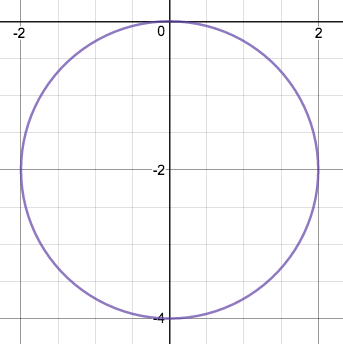
\includegraphics[width = 5 cm, height = 5 cm]{ALEX4.png}
\end{center}
With all this knowledge of the graphs, we can use it to find the area of the graphs.
\section*{Derivatives}
In order to find the derivative, or the slope of a tangent line on a polar function for a specific theta value, we must first build a formula using some knowledge about polar functions. The slope of the tangent line, expressed as $\frac{dy}{dx}$ can also be thought of as $\frac{\frac{dy}{d\theta}}{\frac{dx}{d\theta}}$. These expressions are the change in y and change in x with respect to theta. These measure how y and x individually change as the value of theta changes. We can find equations for these expressions by using our knowledge that in polar equations, $x=r(\theta)cos\theta$ and $y=r(\theta)sin\theta$.\\\\
Let’s take the derivative of x and y with respect to theta.
$$\frac{dx}{d\theta}=cos\theta \cdot \frac{dr}{d\theta}+r(\theta)sin\theta$$
$$\frac{dy}{d\theta}=sin\theta \cdot \frac{dr}{d\theta}+r(\theta)cos\theta$$
Now, let’s substitute these expressions back in to create the formula to find the slope of the tangent line on a polar function.
$$\frac{dy}{dx}=\frac{sin\theta \cdot \frac{dr}{d\theta}+r(\theta)cos\theta}{cos\theta \cdot \frac{dr}{d\theta}+r(\theta)sin\theta}$$
In this formula, $\frac{dr}{d\theta}$ represents the change in the distance to the pole, or the length of r, as the theta value changes. This can be found by taking the derivative of r when r is written as a function. Examples explaining this will be shown below. In some cases, this isn’t even needed because $\frac{dr}{d\theta}$ would be zero, which would cause $\frac{dy}{dx}$ to be $\frac{0}{0}$, or a non-real number. In these cases, we can solve for $\frac{dy}{dx}$ in a much simpler fashion. Let’s try this in example 1.\\\\
\underline{Example 1}
Find $\frac{dy}{dx}$ for the given equation when $\theta=\frac{\pi}{4}$.
$$r=5$$
As we can see, if we took the derivative of r, we’d end up with 0, which would get us that non-real answer that we don’t want. So instead, we should use our knowledge that $x=rcos\theta$ and $y=rsin\theta$ to our advantage. Let’s substitute 5 in for r and then take the derivative of x and y with respect to theta.
$$x=5cos\theta$$
$$\frac{dx}{d\theta}=-5sin\theta$$
$$y=5sin\theta$$
$$\frac{dy}{d\theta}=5cos\theta$$
Let’s rewrite $\frac{dy}{dx}$.
$$\frac{dy}{dx}=\frac{5cos\theta}{-5sin\theta}$$
Now, let’s substitute in $\frac{\pi}{4}$ to find the value of $\frac{dy}{dx}$ there. 
$$\frac{dy}{dx}=\frac{\frac{5\sqrt2}{2}}{-\frac{5\sqrt2}{2}}=-1$$
This makes sense if we look at how the tangent line would behave at $\frac{\pi}{4}$.
\begin{center}
    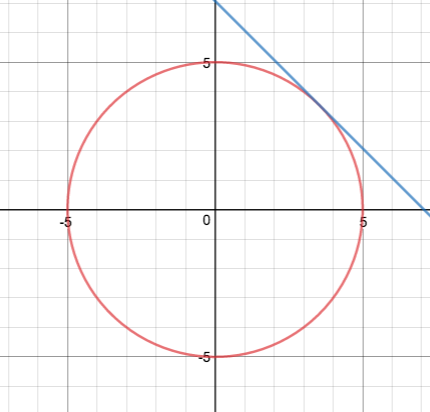
\includegraphics[height=4cm, width=4cm]{Images/negone.png}
\end{center}
\underline{Example 2}
Find the horizontal and vertical tangent lines of the polar equation from example 1 over the interval $0\leq \theta \leq 2\pi$\\\\
Just like we did for parametric equations, to find the horizontal tangent lines, we set the numerator, or $\frac{dy}{d\theta}$  equal to 0. To find vertical tangent lines, we set the denominator equal to zero. Let’s start by finding the horizontal tangent lines.
$$5cos\theta=0$$
$$cos\theta=0$$
So, we know that there are horizontal tangent lines when theta equals $\frac{\pi}{2}$ or $\frac{3\pi}{2}$.
Now let‘s find the vertical tangent lines.
$$-5sin\theta=0$$
$$sin\theta=0$$
So, we know that there are vertical tangent lines when theta equals 0 or $\pi$. To better understand this, let’s look at the tangent lines graphed on the graph of the function below.
\begin{center}
    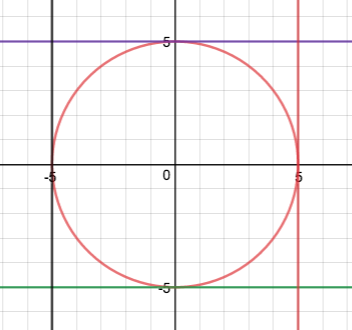
\includegraphics[height=4cm, width=4cm]{Images/stuff.png}
\end{center}
\underline{Example 3}
Write the equation of the tangent line for the polar function $r=2+2cos\theta$ at $\frac{\pi}{2}$.\\\\
This is a problem where we’ll need to find $\frac{dr}{d\theta}$. 
$$\frac{dr}{d\theta}=-2sin\theta$$
Now we can use the formula that we derived earlier to find $\frac{dy}{dx}$.
$$\frac{dy}{dx}=\frac{-2sin^2\theta+(2+2cos\theta)cos\theta}{-2sin\theta cos\theta+(2+2cos\theta)sin\theta}$$
Distribute the cosine and sine in multiplication.
$$\frac{dy}{dx}=\frac{-2sin^2\theta+2cos\theta+2cos^2\theta}{-2sin\theta cos\theta+2sin\theta+2sin\theta cos\theta}$$
Factor out a 2 and simplify the denominator.
$$\frac{dy}{dx}=\frac{cos\theta+cos^2\theta-sin^2\theta}{sin\theta}$$
Replace $cos^2\theta-sin^2\theta$ with $cos(2\theta)$ by using trig identities.
$$\frac{dy}{dx}=\frac{cos\theta+cos2\theta}{sin\theta}$$
Now we'll substitute in $\frac{\pi}{2}$ to find the slope of the tangent line at this point. 
$$\frac{dy}{dx}=\frac{0-1}{1}=-1$$
Now, we have to find our x and y coordinates at $\frac{\pi}{2}$. To do this, we'll have to substitute r into our polar functions $x=rcos\theta$ and $y=rsin\theta$. 
$$x=(2+2cos\theta)cos\theta$$
$$y=(2+2cos\theta)sin\theta$$
Now let's substitute $\frac{\pi}{2}$ in and get our x and y values. 
$$x=(2+0)0=0$$
$$y=(2+2)1=4$$
Let's use these values to write the equation of the tangent line. 
$$y=-1(x+0)+4$$
$$y=-x+4$$
\section*{Area}
Finding the area of Polar equations is actually about the same way we find rectangular area. When we have a rectangular graph and we are finding the area, we think about making thin rectangles that fit into our graph. With polar equations, we want to think about a nice arc cut out of the equation and finding the area of that.\\\\
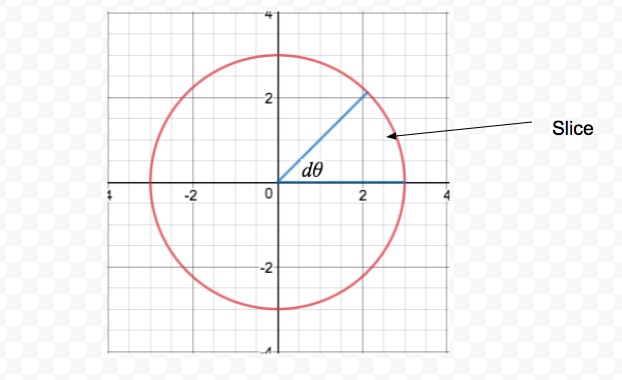
\includegraphics[width = 14 cm, height = 7 cm]{PA1.png}\\
So $d\theta$ is going to represent the change of the angle of that arc and we are going to be squaring the radius and dividing it by 2 in our integral.
$$\frac{1}{2}\int r^2d\theta$$
Let's find the area of the unit circle to prove our relationship. We know it's just going to have a radius of one so lets just find it using the formula, $\pi r^2$ first.\\
$$\pi (1)^2 =area$$
Now let's use our integral with bound from 0 to $2\pi$.
$$\frac{1}{2} \int \limits _0 ^{2\pi} 1^2 d\theta$$
Evaluate.
$$\frac{1}{2}\cdot(\theta)|_0 ^{2\pi}$$
$$\frac{1}{2}\cdot(2\pi)-\frac{1}{2}(0)=\pi$$
As you can see both evaluate to become $\pi$. The formula does give an accurate answer to our polar area. Let's try some more examples. \\\\
\underline{Example Folium}
In order to find the loop nicely we will have to convert to polar form. We are going to use substitutions of $y=r\cdot sin(\theta)$ and $x=r\cdot cos(\theta)$ where $\theta$ is any angle and r is the radius.
$$(r\cdot sin\theta)^3 +(r\cdot cos\theta)^3=3r^2 cos\theta sin\theta$$
$$r^3(cos^3 \theta +sin^3\theta)=3r^2 cos\theta sin\theta$$
$$r=\frac{3 cos\theta sin\theta}{(cos^3 \theta +sin^3\theta)}$$
Now that we have this equation for the polar form, we have to find what angles we're going to use to evaluate over for our integral. Since we know that there is symmetry in the folium lets use that to our advantage. Lets find the area from the angle of 0 to angle $\frac{\pi}{4}$ and multiply it by two. To solve for the area of a polar equation we use the formula of$\frac{1}{2}\cdot \int\limits_a ^b r^2 d\theta$. A and b are two angles in which the area evaluated is in between. Substitute in our values
$$2\cdot \frac{1}{2}\cdot  \int\limits_0 ^{\pi/4} (\frac{3 cos\theta sin\theta}{(cos^3 \theta +sin^3\theta)})^2 d\theta$$
To solve this integral we need to do a bit of variable manipulation because it would be easier to solve something with a nice u substitution. So lets mess a bit with the radius.
$$r=\frac{3 cos\theta sin\theta}{(cos^3 \theta +sin^3\theta)}$$
First multiply by $sec^3(\theta)$ by both the top and bottom to create a new radius of...
$$r=\frac{3 cos\theta sin\theta}{(cos^3 \theta +sin^3\theta)} \cdot \frac{sec^3(\theta)}{sec^3(\theta)}=\frac{3sec\theta tan\theta}{1+tan^3 \theta}$$
Substitute this in to our integral.
$$ \int\limits_0 ^{\pi/4} (\frac{3sec\theta tan\theta}{1+tan^3 \theta})^2 d\theta$$
Then square out the radius.
$$ \int\limits_0 ^{\pi/4} \frac{9sec^2\theta tan^2\theta}{(1+tan^3 \theta)^2} d\theta$$
Create a u substitution of $tan^3\theta + 1$.
$$u=tan^3 \theta +1$$
$$du=3sec^2\theta tan^2\theta d\theta$$
Also change your bounds by substituting them  into $tan^3 \theta$
$$tan^3(0)+1=0+1=1$$
$$tan^3(\pi /4)+1=(\frac{\sqrt{2}/2}{\sqrt{2}/2})^3+1=2$$
Substitute in your u-sub with new bounds.
$$ \int\limits_1 ^{2} \frac{3}{(u)^2} du$$
Finish integrating and solve for your bounds.
$$\frac{-3}{u}|_1 ^2$$
$$\frac{-3}{2}+\frac{3}{1}=\frac{3}{2}$$
\\
The area is 3/2 units squared.\\\\
\underline{Example Between Curves}
Let's find the area inside the polar curve $r=2+2sin\theta)$ and the polar curve $r=2$. We first need to look at the graph of both of these together and locate region needed.\\
\begin{center}
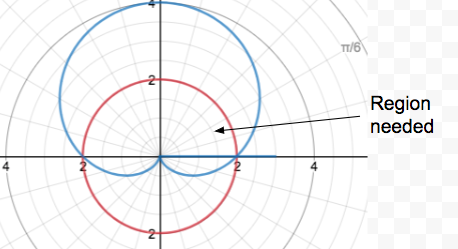
\includegraphics[width = 14 cm, height = 7 cm]{JOSH3.png}
\end{center}
Notice how the graphs intersect at two points. These points are going to be bounds for our integral. So let's set the polar equations equal to each other and solve for our points.
$$2=2+2sin\theta$$
$$0=sin\theta$$
$$\theta=0,\pi,2\pi$$
Now that we have these points we can create an integral using what we know about the graph. First we're going to find the area of half of the circle then add the area from the angles $\pi$ to $2\pi$ of the cartiod.
$$\frac{1}{2}\cdot \pi 2^2 + \frac{1}{2}\int\limits_\pi ^{2\pi}(2+2sin\theta)^2 d\theta$$
Evaluate the integral.
$$2\pi +\frac{1}{2}(\int\limits_\pi ^{2\pi}4+8sin\theta+4sin^2\theta d\theta)$$
$$2\pi +2(\int\limits_\pi ^{2\pi}1+2sin\theta+sin^2\theta  d\theta)$$
Let's isolate the integral and solve for its anti-derivative then we can add $2\pi$ later.
$$2(\int\limits_\pi ^{2\pi}1+2sin\theta+sin^2\theta d\theta)$$
$$\int\limits_\pi ^{2\pi}2d\theta + 4\int\limits_\pi ^{2\pi}sin\theta d\theta +2\int\limits_\pi ^{2\pi}sin^2\theta d\theta$$
Now in order to evaluate $sin^2 \theta$ we can make a substitution of $sin^2 \theta=\frac{1-cos2\theta}{2}$.
$$\int\limits_\pi ^{2\pi}2d\theta + 4\int\limits_\pi ^{2\pi}sin\theta d\theta +2\int\limits_\pi ^{2\pi}\frac{1-cos2\theta}{2} d\theta$$
Now evaluate.
$$\int\limits_\pi ^{2\pi}2d\theta + 4\int\limits_\pi ^{2\pi}sin\theta d\theta +2\int\limits_\pi ^{2\pi}\frac{1-cos2\theta}{2} d\theta$$
$$2\theta - 4cos\theta +\theta-\frac{1}{2}sin2\theta|_\pi^{2\pi}$$
$$3\theta - 4cos\theta-\frac{1}{2}sin2\theta|_\pi^{2\pi}$$
$$6\pi-3\pi-4-4=3\pi-8$$
Then add $2\pi$
$$5\pi - 8$$
This process is just one of many tricks. Another way to solve polar areas is through symmetry. This way makes it sometimes eaiser to evaluate your answers.
\ssection{Arc Length}
\section*{Parametric}
Parametric arc length is found by manipulating the distances formula because arc length is the distance of the arc that is being measured. In this graph we see that a point to another point is $y_2-y_1$ which is $dy$ and $x_2-x_1$ which is $dx$ but because this is in parametric form it is $\frac{dy}{dt}$ and $\frac{dx}{dt}$. The distance formula is $$d=\sqrt{(x_2-x_1)^2+(y_2-y_1)^2}$$ and when we substitute the pieces for their parametric counterparts, we get the parametric form which makes up the equation for arc length because they both measure distance. So that means that it turns into $=\sqrt{(\frac{dx}{dt})^2+(\frac{dy}{dt})^2}$. But we can't stop there because this formula just measures the distance of lines which will give an approximate value and not a exact curve which is showed in this image \begin{center}
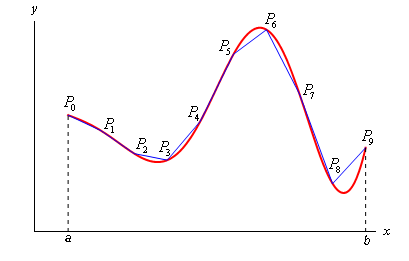
\includegraphics[width = 7 cm, height = 5 cm]{arclength.png}
\end{center}
To do that we will have to take a sum over an interval so we can add up all the segments ad to find a more exact distance of the curve because there will be more steps. And then you have to take the limit of that to infinity to see what the integral is approaching to see that the curve is continuous and to make each number more exact and then you can use the definition of a definite integral to turn it into a integral making the arc length formula being this with arc length $$=\int_{a}^{b}\sqrt{(\frac{dx}{dt})^2+(\frac{dy}{dt})^2}dt$$ This formula can then be manipulated to find a polar form arc length by substituting in trig and rectangular can be found by manipulating the functions and turning the inside into dx and dy instead of $\frac{dx}{dt}$ and $\frac{dy}{dt}$  
An example of finding arc length with parametric equations is with the equations of $x=cost$ and $y=sint$ which are the equations of the unit circle so it will be done over the interval of 0 to $2\pi$ and before we substitute we have to find their derivative because that is what the formula uses \\When these equations are substituted into the equation you get this $$\int_{0}^{2\pi}\sqrt{-sint)^2+(cost)^2}dt$$ which just simplifies down to $$\int_{0}^{2\pi}1dt$$ which turns into t over 0 to $2\pi$ which just turns into $2\pi$ which is the arc length of the unit circle.
\section*{Rectangular}
The rectangular formula is pretty easy to get. All you do is use the parametric form you got which is...
$$\int\sqrt{(\frac{dx}{dt})^2+(\frac{dy}{dt})^2}dt$$
and convert by eliminating the parameter which means dx is going to be equal to dt.
$$\int\sqrt{(\frac{dx}{dx})^2+(\frac{dy}{dx})^2}dx$$
simplify
$$\int\sqrt{1+(\frac{dy}{dx})^2}dx$$
Let's use the equation $y=x^2$ as our example with bounds of $-2\leq x\leq 2$.

$$y=x^2$$
$$\frac{dy}{dx}=2x$$
substitute into our formula and solve with bounds

$$\int\limits_{-2}^2\sqrt{1+(2x)^2}dx$$
$$\int\limits_{-2}^2\sqrt{1+4x^2}dx$$
We will have to use a calculator because it cant be solved using any tricks. SO your answer will be about 9.294.
\section*{Polar}
The polar formula is the easiest way to find the arc length of a polar equation. The most difficult part about it is deriving the formula. Let's try doing that, so we know where the simple formula really comes from.\\\\
Our goal is to use our knowledge of the parametric arc length formula and manipulate it to help us find the polar arc length formula. So, to do that, we'll start off using the equations of x and y in terms of r and $\theta$ so that we can manipulate these to get the end formula in terms of r.
$$x=rcos\theta$$
$$y=rsin\theta$$
Now we'll want to find $\frac{dx}{d\theta}$ and $\frac{dy}{d\theta}$ to arrange the formula like the parametric formula.
$$\frac{dx}{d\theta}=r'cos\theta -rsin\theta$$
$$\frac{dx}{d\theta}=\frac{dr}{d\theta}cos\theta -rsin\theta$$
$$\frac{dy}{d\theta}=r\sin\theta +rcos\theta$$
$$\frac{dy}{d\theta}=\frac{dr}{d\theta}sin\theta +rcos\theta$$
Now we want to rewrite it as $(\frac{dx}{d\theta})^2+(\frac{dy}{d\theta})^2$ to get it close to the parametric form, which is written as $(\frac{dx}{dt})^2+(\frac{dy}{dt})^2$. Substitute in $\frac{dx}{d\theta}$ and $\frac{dy}{d\theta}$ and solve.
$$(\frac{dx}{d\theta})^2+(\frac{dy}{d\theta})^2=(\frac{dr}{d\theta}cos\theta -rsin\theta)^2+(\frac{dr}{d\theta}sin\theta +rcos\theta)^2$$
$$=(\frac{dr}{d\theta})^2cos^2\theta-2r\frac{dr}{d\theta}cos\theta sin\theta+r^2sin^2\theta+(\frac{dr}{d\theta})^2sin^2\theta+2r\frac{dr}{d\theta}cos\theta sin\theta+r^2cos\theta$$
$$=(\frac{dr}{d\theta})^2(cos^2\theta+sin^2\theta)+r^2(cos^2\theta+sin^2\theta)$$
Simplify using trig identities.
$$=(\frac{dr}{d\theta})^2+r^2$$
Now we have to remember that this is another way of writing the parametric formula, but only in terms of r, so we have to write this the same way as the parametric formula.
$$\int_{a}^{b}\sqrt(\frac{dr}{d\theta})^2+r^2 d\theta$$
Now let’s try this formula on a problem.
First let’s try it on the unit circle to make sure it works, since we know how to calculate the circumference of a circle with a formula $circumference=2\pi r$.\\\\
\underline{Example 1}
$$r=1$$
$$\frac{dr}{d\theta}=0$$
$$\int_{0}^{2\pi}\sqrt1^2+0^2 d\theta$$
$$\int_{0}{2\pi}1d\theta$$
$$\theta\vert_{0}^{2\pi}=2\pi$$
If we use the circumference formula, we get the same thing.
$$2\pi \cdot1=2\pi$$
This proves that the formula that we found is correct. Now let’s try using it on a more difficult problem.\\\\
\underline{Example 2}
Find the circumference of the cardiod from $\frac{\pi}{2}$ to $\frac{3\pi}{2}$.
$$r=3+2sin(\theta)$$ 
$$\frac{dr}{d\theta}=2cos(\theta)$$
$$\int_{\frac{\pi}{2}}^{\frac{3\pi}{2}}\sqrt(3+2sin\theta)^2+(2cos\theta)^2$$
$$\int_{\frac{\pi}{2}}^{\frac{3\pi}{2}}\sqrt9+12sin\theta+4sin^2\theta+4cos^2\theta d\theta$$
$$\int_{\frac{\pi}{2}}^{\frac{3\pi}{2}}\sqrt9+12sin\theta+4$$
$$\int_{\frac{\pi}{2}}^{\frac{3\pi}{2}}\sqrt13+12sin\theta d\theta = 21.01$$
\ssection{Vectors}
\section*{Unit Vectors}
A vector is a directed line segment with a direction, or angle, and a length, or a magnitude. We'll talk about these properties later. Vectors can either be written as:
$<5,-3>$ or $5i-3j$. Both of these express the same thing. For this specific vector, it would look like:
\begin{center}
    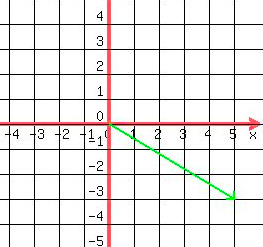
\includegraphics[width=4cm, height=4cm]{Images/unit.png}
\end{center}
As we can see, unit vectors work just like x and y coordinates. When graphing them, the number in front of the i or the first number in the caret notation is the x component and the number in front of the j or the second number in the caret notation is the y component. 
\section*{Magnitude and Direction}
When a vector is formed you are given a tail and then an head. This segment starts at the tail and ends with the head like this...\\
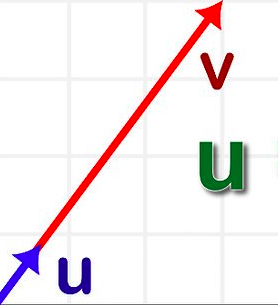
\includegraphics[width = 7 cm, height = 5 cm]{norm.png}
\\\\
As you can see at u there is a tail and at v there is a head. This shows the direction of which the vector is going to. The distance or magnitude of the vector is often identified like this $||\overrightarrow{v}||$ where $\overrightarrow{v}$ is a vector. In order to find the magnitude you square each component and then add the up and then square root the sum. For example...
$$\overrightarrow{v}=<3,4>$$
$$||c||=\sqrt{3^2 +4^2}=5$$
so your answer will be 5. IF there is more then two components your process will still be the same for finding the magnitude.\\\\
\section*{Addition, Subtraction, Dot Product, Cross Product}
\underline{Addition}
Adding vectors is as simple as basic addition. Let's look at the diagram below and use it to explain how we add vectors.
\begin{center}
    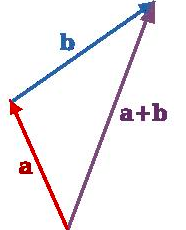
\includegraphics[width=4cm, height=4cm]{Images/addvector.png}
\end{center}
To add vectors, we have to place the vectors end to end like we did here with \overrightarrow{a} and \overrightarrow{b}. Then, to figure out how we get the sum of those vectors, we start at the beginning of the first vector (\overrightarrow{a}), and we move along it to its end. This is going to be the first vector in our sum. Since the end of our first vector is also the beginning of the second vector, we pick up where we left off at the end of the first vector and we follow along the second vector (\overrightarrow{b}), all the way to its head. This will be the second vector in our sum. So, the new vector created in this example would be \overrightarrow{a}+\overrightarrow{b}.\\\\
The new vector that's created has its tail at the same point as the tail of \overrightarrow{a} and its head is at the same point that \overrightarrow{b} has its head. If we were looking at a vector that is $a=<a_{1},a_{2}>$ and another that is $b=<b_{1},b_{2}>$, the addition of \overrightarrow{a}+\overrightarrow{b} would be:
$$<a_{1}+b_{1},a_{2}+b_{2}>$$\\\\
Now, let's try this in an example.\\\\
\underline{Example 1}
$$\overrightarrow{v}=<1,3>$$
$$\overrightarrow{u}=<2,-4>$$
Find \overrightarrow{v}+\overrightarrow{u}.
$$\overrightarrow{v}+\overrightarrow{u}=<1+2,3-4>=<3,-1>$$
It's that simple to find the sum of two vectors.\\\\
\underline{Subtraction}\\
Now, let's try seeing what happens when we subtract two vectors.
\begin{center}
    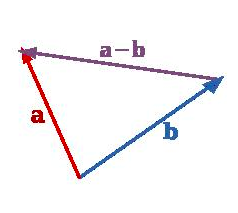
\includegraphics[width=4cm, height=4cm]{Images/subvector.png}
\end{center}
In this case, we'd place the tails of the two vectors together and we'd start off following the second vector, \overrightarrow{b}. Starting at the head of \overrightarrow{b}, we'd draw a vector from this point to the head of \overrightarrow{a}. This may be backwards from what we'd think, but in this case, \overrightarrow{b} would be the second part of the subtraction and \overrightarrow{a} would be the first. So, if we had a vector $a=<a_{1},a_{2}>$ and another that's $b=<b_{1},b_{2}>$, the subtraction of \overrightarrow{a}-\overrightarrow{b} would be:
$$<a_{1}-b_{1},a_{2}-b_{2}>$$
Now, let's try an example.
$$\overrightarrow{v}=<-7,8>$$
$$\overrightarrow{u}=<3,-4>$$
Find \overrightarrow{v}-\overrightarrow{u}.
$$\overrightarrow{v}-\overrightarrow{u}=<-7-3,8--4>=<-10,12>$$
Subtracting vectors is that simple.
\underline{Dot Product}\\
The idea of the dot product is to multiply each group of components and add the all up to see a relationship. This relationship is orthogonal which is like perpendicular but in terms of vectors. So the formula is going to be...
$$\overrightarrow{v}=<a_1 ,b_1, c_1,...>$$
$$\overrightarrow{u}=<a_2 ,b_2, c_2,...>$$
$$\overrightarrow{v}\cdot \overrightarrow{u}=a_1 a_2 +b_1 b_2 +c_1 c_2+...$$
Let's try an example.
$$\overrightarrow{v}=<5 ,-2,>$$
$$\overrightarrow{u}=< 2,5,>$$
$$\overrightarrow{v}\cdot \overrightarrow{u}=5\cdot 2 -2\cdot5=0$$
Since the dot product came out to zero the two vectors are orthogonal to each other. This idea is done with all components. Dot product is also commutative so it doesn't matter which way you put the vectors. Also $cos\theta=\frac{\overrightarrow{v}\cdot \overrightarrow{u}}{||\overrightarrow{v}|| || \overrightarrow{u}||}$
This means that cosine of an angle is equal to the dot product over the multiplication of the magnitudes of the two vectors. This angle is in between vector u and v.
\\\\\underline{Cross Product}\\
The cross product is not really like the dot at all. What happens is that you create a new vector that is perpendicular to the other two. The vector's components are created using the idea behind matrices and has to have a min of three components. The formula is below...
$$\overrightarrow{v}=<a_1 ,b_1, c_1>$$
$$\overrightarrow{u}=<a_2 ,b_2, c_2>$$
$$\overrightarrow{v}\times \overrightarrow{u}=<b_1 c_2-b_2 c_1,-(a_1 c_2-a_2 c_1),a_1 b_2-a_2 b_1>$$
Let's try an example then test if it truly is perpendicular. 
$$\overrightarrow{v}=< 7,1,6 >$$
$$\overrightarrow{u}=< 5,2,0 >$$
$$\overrightarrow{v}\times \overrightarrow{u}=<0-12,30,14-5>=<-12,30,9>$$
Now let's do dot product to see if it is orthogonal.
$$(\overrightarrow{v}\times \overrightarrow{u})\cdot \overrightarrow{u}=-12\cdot5+2\cdot30+0\cdot9=-60+60=0$$
So the relationship is true and the cross product works. Note that the cross product does depend on the order you put the two vectors in. Also anytime there is two components for a vector just add a third y saying the new one is equal to 0 like this...
$$\overrightarrow{v}=< 7,1>=<7,1,0>$$
Tips like this can help you grind out the whole product.
\section*{Normalized Vectors, Orthogonal Vectors, Area of a Parallelogram} 
Normalized vector are vectors that are going in the same directions but the normalized vector has a magnitude (length) of 1. You do this by dividing the vector by it's magnitude which will form a vector going in the same direction and will have a magnitude of 1 because the magnitude will be the length of the vector, and then the new vector will look like this \begin{center}
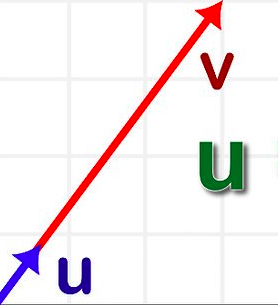
\includegraphics[width = 7 cm, height = 5 cm]{norm.png}
\end{center} U as you can see is the normalized vector as it only has a magnitude of 1
\\Orthogonal (perpendicular) vectors are  vectors that when a dot product is done between them that equals 0. This is true because if the dot product is done than we will see that there slope values will equal 0 because they are perpendicular. they look like this \begin{center}
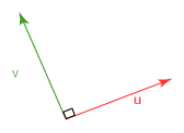
\includegraphics[width = 7 cm, height = 5 cm]{orthogonal.png}
\end{center} \\The area of a parallelogram is found by multiplying base times height which can also be modeled as the magnitude of the dot product of two vectors this can be proven because when you take account of the the angle which you find as being $sin\theta=\frac{h}{||v||}$ the parallelogram is modeled here
\begin{center}
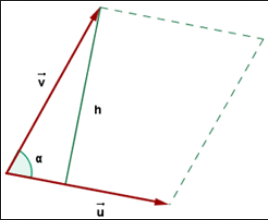
\includegraphics[width = 7 cm, height = 5 cm]{vector.png}
\end{center}
we can manipulate are last equation to see that $h=sin\theta||\vec{v}||$ and when we multiply that by the base we get that the area of a parallelogram is this $||\vec{v}||||\vec{u}||sin\theta$
and this can re written in other words as $$||\vec{u}X\vec{v}||$$ 
All of these have pretty simple equations, so lets have an example for each of these three.\\\\
\underline{Example 1} normalize the vector $$\vec{i} + \sqrt{3}\vec{k}$$ 
we first have to find the magnitude of it which is just $\sqrt{1^2+(\sqrt{3})^2}$ which is 2, so the normalized vector is $$\frac{1+\sqrt{3}}{2}$$\\
\underline{Example 2} find a vector orthogonal to one with the equation of -2i-5j+1k. with most of these its just guess and check to find an orthogonal vector because there can be many choices lets start with multiplying -2 by 3 and -5 by -2 which adds up to 4 and then we have to multiply the 1 by -4 so that together they equal 0. So therefore an orthogonal line is 3i-2j+-4k\\\\
\underline{Example 3} Find the area of this parallelogram with $\vec{u}=2i+3j+4k $ and $\vec{v}=5i+6j+7k $
All we have to do is take the magnitude of the cross product so that means we take $(3*7-4*6)i-(2*7-5*4)j+(2*7-3*5)k$ which is $-3i+6j-k$ and when we take the magnitude we get $$\sqrt{(-3)^2+(6)^2+(-k)^2}$$ which simplifies to $$\sqrt{46}$$
\section*{Velocity-Acceleration-Total Distance Traveled}
A velocity vector represents the rate of change of the position of an object. The magnitude of a velocity vector gives the speed of an object while the vector direction gives its direction. Velocity vectors can be added or subtracted. It is the derivation of position with velocity being displacement over time and average velocity being the change in position over time. Acceleration vectors show the rate at which an object changes its velocity. An object is accelerating if it is changing its velocity. It is derived again from the velocity vector over time again, and the average acceleration is the change in velocity over time. The total distance traveled is the measure found by adding up all of the vectors and each of there distances traveled which can be found by adding up all the positions during a time period or by taking the integral of a velocity vector during a time period. Here is example of a table of vectors that could be found 
\begin{center}
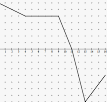
\includegraphics[width = 7 cm, height = 5 cm]{vectors.png}
\end{center}
Now for some examples\\\\
Suppose a train moves northwest out of a station at a speed of 200 km/hr in a direction of 100 degrees (i.e., 30 degrees north of west). The border is located a distance of 1000 km due north of the train. Calculate the time when the train will cross the border. The northern vector is $200*sin(100)$ which is 196 km/hour and since $t=\frac{distance north}{vector}$ which is $\frac{1000}{196}=5.1$ so it takes 5.1 hours.\\\\
\underline{example 2}\\\\
Given the distance parametric equations $x(t)=7t^3+t^2$ and $y(t)=t^4-5t^2$ find the velocity vector. This problem is very easy to solve for. We just find the velocity for each parametric equation and put into a vector like this $v(t)=<x'(t),y'(t)>$. So let's start.
$$x'(t)=4t^3 -10t$$
$$y'(t)=21t^2 +2t$$
$$v(t)=<4t^3 -10t,21t^2 +2t>$$
With this we can solve for when the particle in motion is resting or at what velocities it can reach.
\end{document}
